\documentclass[final]{cpecmu}

%% This is a sample document demonstrating how to use the CPECMU
%% project template. If you are having trouble, see "cpecmu.pdf" for
%% documentation.

\projectNo{ S040-1}
\acadyear{2021}

\titleTH{วงเวียน : แอพพลิเคชันรีวิว}
\titleEN{Wongwien : A Review Application}

\author{นายวริทธิ์ธร อุตตะมา}{Waritthon Auttama}{610610612}

\cpeadvisor{lachana}
\cpecommittee{sakgasit}
\cpecommittee{kampol}
% \committee{รศ.ดร.\,นิพนธ์ ธีรอำพน}{Assoc.\,Prof.\,Nipon Theera-Umpon, Ph.D.}

%% Some possible packages to include:
\usepackage[final]{graphicx} % for including graphics

%% Add bookmarks and hyperlinks in the document.
\PassOptionsToPackage{hyphens}{url}
\usepackage[colorlinks=true,allcolors=Blue4,citecolor=red,linktoc=all]{hyperref}
\def\UrlFont{\thaifonttt}

%% Needed just by this example, but maybe not by most reports
\usepackage{afterpage} % for outputting
\usepackage{pdflscape} % for landscape figures and tables. 

%% Some other useful packages. Look these up to find out how to use
%% them.
% \usepackage{natbib}    % for author-year citation styles
% \usepackage{txfonts}
% \usepackage{appendix}  % for appendices on a per-chapter basis
% \usepackage{xtab}      % for tables that go over multiple pages
% \usepackage{subfigure} % for subfigures within a figure
% \usepackage{pstricks,pdftricks} % for access to special PostScript and PDF commands
% \usepackage{nomencl}   % if you have a list of abbreviations

%% if you're having problems with overfull boxes, you may need to increase
%% the tolerance to 9999
% \tolerance=9999

\bibliographystyle{plain}
% \bibliographystyle{IEEEbib}

% \renewcommand{\topfraction}{0.85}
% \renewcommand{\textfraction}{0.1}
% \renewcommand{\floatpagefraction}{0.75}

%% Example for glossary entry
%% Need to use glossary option
%% See glossaries package for complete documentation.
\ifglossary
  \newglossaryentry{lorem ipsum}{
    name=lorem ipsum,
    description={derived from Latin dolorem ipsum, translated as ``pain itself''}
  }
\fi

%% Uncomment this command to preview only specified LaTeX file(s)
%% imported with \include command below.
%% Any other file imported via \include but not specified here will not
%% be previewed.
%% Useful if your report is large, as you might not want to build
%% the entire file when editing a certain part of your report.
% \includeonly{chapters/intro,chapters/background}

\begin{document}
\maketitle
\makesignature

\ifproject
\begin{abstractTH}
% เขียนบทคัดย่อของโครงงานที่นี่

การเขียนรายงานนี้เป็นส่วนหนึ่งของการทําโครงงานวิศวกรรมคอมพิวเตอร์ ได้ทำออกมาในรูปแบบของ Application โดยอุปกรณ์เน้นการทำงานบนโทรศัพท์มือถือ (android) เป็นหลัก ซึ่งโครงงานนี้จัดขึ้นเพื่อเป็นตัวเลือกหนึ่งที่ใช้ในการประกอบการตัดสินใจ หรือไขข้อสงสัย ผ่านระบบของการรีวิว กระดานกระทู้ และการปรึกษาพูดคุยเพื่อต้องการความช่วยเหลือ โดยแอพพลิเคชั่นสามารถรองรับการเข้าใช้งานโดยผ่านแพลตฟอร์มอื่น และสามารถช่วยค้นหาข้อมูลที่ต้องการได้ง่าย การใช้งานไม่ซับซ้อนสามารถเข้าใช้งานได้ไม่ยากเหมาะกับทุกเพศทุกวัย

% การเขียนรายงานเป็นส่วนหนึ่งของการทำโครงงานวิศวกรรมคอมพิวเตอร์
% เพื่อทบทวนทฤษฎีที่เกี่ยวข้อง อธิบายขั้นตอนวิธีแก้ปัญหาเชิงวิศวกรรม และวิเคราะห์และสรุปผลการทดลองอุปกรณ์และระบบต่างๆ
% \enskip อย่างไรก็ดี การสร้างรูปเล่มรายงานให้ถูกรูปแบบนั้นเป็นขั้นตอนที่ยุ่งยาก
% แม้ว่าจะมีต้นแบบสำหรับใช้ในโปรแกรม Microsoft Word แล้วก็ตาม
% แต่นักศึกษาส่วนใหญ่ยังคงค้นพบว่าการใช้งานมีความซับซ้อน และเกิดความผิดพลาดในการจัดรูปแบบ กำหนดเลขหัวข้อ และสร้างสารบัญอยู่
% \enskip ภาควิชาวิศวกรรมคอมพิวเตอร์จึงได้จัดทำต้นแบบรูปเล่มรายงานโดยใช้ระบบจัดเตรียมเอกสาร
% \LaTeX{} เพื่อช่วยให้นักศึกษาเขียนรายงานได้อย่างสะดวกและรวดเร็วมากยิ่งขึ้น
\end{abstractTH}

\begin{abstract}
The abstract would be placed here. It usually does not exceed 350 words
long (not counting the heading), and must not take up more than one (1) page
(even if fewer than 350 words long).

Make sure your abstract sits inside the \texttt{abstract} environment.
\end{abstract}

\iffalse
\begin{dedication}
This document is dedicated to all Chiang Mai University students.

Dedication page is optional.
\end{dedication}
\fi % \iffalse

\begin{acknowledgments}
Your acknowledgments go here. Make sure it sits inside the
\texttt{acknowledgment} environment.

\acksign{2020}{5}{25}
\end{acknowledgments}%
\fi % \ifproject

\contentspage

\ifproject
\figurelistpage

\tablelistpage
\fi % \ifproject

% \abbrlist % this page is optional

% \symlist % this page is optional

% \preface % this section is optional


\pagestyle{empty}\cleardoublepage
\normalspacing \setcounter{page}{1} \pagenumbering{arabic} \pagestyle{cpecmu}

\chapter{\ifenglish Introduction\else บทนำ\fi}

\section{\ifenglish Project rationale\else ที่มาของโครงงาน\fi}

การเรียนรู้เรื่องราวต่างๆเกี่ยวกับมหาวิทยาลัยนั้นทําได้หลายวิธี แต่เมื่อพูดถึงการใช้ชีวิตแล้วการรีวิวก็ถือว่าเป็นการถ่ายทอด
ประสบการณ์ที่ดีวิธีหนึ่งนอกจากนี้ยังอาจเป็นแนวทางการใช้ชีวิตและช่วยในการแก้ไขปัญหาหรือให้ข้อมูลข้อคิดเห็นและประสบการณ์เกี่ยวกับ
เรื่องราวที่คนกลุ่มหนึ่งให้ความสนใจร่วมกัน เช่น วิชา ร้าน อาหาร เป็นต้น

การรีวิวสิ่งต่างๆที่มีประโยชน์กับนักศึกษามหาวิทยาลัยเชียงใหม่นั้นไม่ได้มีการรวบรวมไว้ทําให้มีการกระจายไปในแพลตฟอร์มต่างๆ
ประกอบกับแต่ละแพลตฟอร์มก็มีข้อจํากัดแตกต่างกันไป อย่างเช่น ระบบที่ใหญ่ของแอพโซวเชียว เช่น facebook ทำให้การค้นหารีวิวนั้นพบเจอ
ได้ยาก ส่วนใหญ่จะพบเจอแต่กลุ่มรีวิวสินค้ามากกว่า รีวิวแนวประสบการณ์ twitter ก็ส่วนใหญ่ที่พบเจอเป็นแนวข่าว pantip ส่วนใหญ่ที่พบเจอ
เป้นแนวกระทู้ถามตอบ พบเจอรีวิวค่อนข้างน้อย เป็นต้น ทําให้การเข้าถึงรีวิวนั้นค่อนข้างยากต้องเสียเวลาพอสมควร แอพพลิเคชันนี้ช่วย
แก้ปัญหาให้ช่วยเป็นอีกตัวเลือกของการีวิวที่ทำให้รีวิวมีการเก็บรวบรวมไว้ให้มีระเบียบมากขึ้น เพื่อให้ค้นหาได้ง่ายด้วยการใช้คำนวน การแบ่ง
หมวดหมู่ แท็กต่างๆในการร่วมกันค้นหา

ผู้พัฒนาได้มองเป็นปัญหาดังกล่าวจึงได้พัฒนาแอปพลิเคชันนี้ขึ้น เพื่อเพิ่มช่วยเสริมการเรียนรู้และเข้าใจการใช้ชีวิตในมหาวิทยาลัยแก่
นักศึกษาและคนที่สนใจ รวมถึงการแก้ไขปัญหา ข้อสงสัยต่างๆ ผ่านการรีวิวที่มีการแยกหมวดหมู่เพื่อเข้าถึงได้ง่ายต่อการค้นหาและสามารถการ
สร้างกระทู้สอบถามเพื่อขอความช่วยเหลือ

โดยทางผู้พัฒนาหวังว่าแอปพลิเคชันนี้จะช่วยในการให้ความรู้และช่วยในการประกอบการตัดสินใจต่างๆ
ได้ง่ายขึ้นผ่านการรีวิวและคําแนะนําจากคนที่มีประสบการณ์หรือมีความรู้ในเรื่องนั้นๆ

\section{\ifenglish Objectives\else วัตถุประสงค์ของโครงงาน\fi}
\begin{enumerate}
    \item เพื่อเป็นสื่อกลางในการถ่ายทอดการรีวิวต่างๆ
    \item เพื่อช่วยอำนวนความสะดวกในการเป็นสื่อกลางในการสอบถาม
    \item เพื่อเป็นสื่อกลางในการติดต่อสื่อสารระหว่างบุคคล
\end{enumerate}

\section{\ifenglish Project scope\else ขอบเขตของโครงงาน\fi}

\subsection{\ifenglish Hardware scope\else ขอบเขตด้านฮาร์ดแวร์\fi}
\begin{enumerate}
    \item รองรับบนโทรศัพท์มือถือแอนดรอยด์
\end{enumerate}
\subsection{\ifenglish Software scope\else ขอบเขตด้านซอฟต์แวร์\fi}
\begin{enumerate}
    \item สามารถเข้าใช้บริการโดยผ่านแฟตฟอร์มอื่นๆ ( facebook,google,email )
    \item สามารถเข้าไปอ่านรีวิว ค้นหารีวิวจากคําค้นหาหรือค้นหาโดยหมวดหมู่ รวมถึงการให้คะแนนรีวิว
    \item สามารถสร้างการรีวิว
    \item สามารถเข้าไปอ่านคําถามที่น่าสนใจ ตอบคําถาม รวมถึงการสร้างกระทู้สอบถามเพื่อไขข้อสงสัย
    \item สามารถติดต่อสื่อสารระหว่างบุคคลเพื่อขอคําแนะนําต่างๆ
\end{enumerate}
\section{\ifenglish Expected outcomes\else ประโยชน์ที่ได้รับ\fi}
\begin{enumerate}
    \item  ช่วยในการประกอบการตัดสินใจต่างๆ
    \item  ช่วยในการเป็นสื่อกลางในการสอบถามระหว่างผู้สงสัยกับผู้ที่มีความรู้
    \item เป็นช่องทางในการติดต่อสื่อสารระหว่างบุคคล
\end{enumerate}
\section{\ifenglish Technology and tools\else เทคโนโลยีและเครื่องมือที่ใช้\fi}

\subsection{\ifenglish Hardware technology\else เทคโนโลยีด้านฮาร์ดแวร์\fi}
\begin{enumerate}
    \item โทรศัพท์แอนดรอยด์
\end{enumerate}
\subsection{\ifenglish Software technology\else เทคโนโลยีด้านซอฟต์แวร์\fi}
\begin{enumerate}
    \item Figma:สําหรับออกแบบตัวแอปพลิเคชัน  
    \item Android studio:พัฒนาแอนดรอยด์แอปพลิเคชัน
    \item Firebase:จัดการฐานข้อมูล การเข้าใช้บริการ
    \item app.diagrams.net:ออกแบบ user diagrams
    \item lucidchart: ออกแบบ schema database
    \item google cloud platform: เชื่อมต่อ google map api
    \item developers facebook: เชื่อมต่อ facebook api สำหรับการ login
\end{enumerate}
\section{\ifenglish Project plan\else แผนการดำเนินงาน\fi}

\begin{plan}{7}{2021}{1}{2022}
    \planitem{7}{2021}{8}{2021}{ศึกษาปัญหา ความต้องการ และรวบรวมข้อมูล}
    \planitem{7}{2021}{8}{2021}{ศึกษาภาษาและเครื่องมือที่ใช้ในการเขียนแอพพลิเคชัน}
    \planitem{8}{2021}{9}{2021}{กําหนดขอบเขตและวางแผนการดําเนินงาน}
    \planitem{8}{2021}{11}{2021}{ออกแบบ UX/UI}
    \planitem{8}{2021}{2}{2022}{พัฒนาแอพพลิเคชัน}
    \planitem{1}{2022}{2}{2022}{เขียนเอกสารรายงาน}
\end{plan}

% \section{\ifenglish Roles and responsibilities\else บทบาทและความรับผิดชอบ\fi}
% อธิบายว่าในการทำงาน นศ. มีการกำหนดบทบาทและแบ่งหน้าที่งานอย่างไรในการทำงาน จำเป็นต้องใช้ความรู้ใดในการทำงานบ้าง

% \section{\ifenglish%
% Impacts of this project on society, health, safety, legal, and cultural issues
% \else%
% ผลกระทบด้านสังคม สุขภาพ ความปลอดภัย กฎหมาย และวัฒนธรรม
% \fi}

% แนวทางและโยชน์ในการประยุกต์ใช้งานโครงงานกับงานในด้านอื่นๆ รวมถึงผลกระทบในด้านสังคมและสิ่งแวดล้อมจากการใช้ความรู้ทางวิศวกรรมที่ได้

\chapter{\ifenglish Background Knowledge and Theory\else ทฤษฎีที่เกี่ยวข้อง\fi}
 การทําโครงงาน เริ่มต้นด้วยการศึกษาค้นคว้า ทฤษฎีที่เกี่ยวข้อง หรือ งานวิจัย/โครงงาน ที่เคยมีผู้นําเสนอ
ไว้แล้ว ซึ่งเนื้อหาในบทนี้ก็จะเกี่ยวกับการอธิบายถึงสิ่งที่เกี่ยวข้องกับโครงงาน เพื่อให้ผู้อ่านเข้าใจเนื้อหาในบท
ถัดๆ ไปได้ง่ายขึ้น
\section{Mobile operating systems}
\subsection{ระบบปฎิบัติการแอนดรอยด์(Android OS)}
\subsubsection{ประวัติและความเป็นมาของระบบปฏิบัติการแอนดรอยด์}

 เริ่มต้นระบบปฏิบัติการแอนดรอยด \cite{android} ถูกพัฒนามาจากบริษัท แอนดรอยด์(Android Inc.) เมื่อปี
พ.ศ 2546 โดยมีนาย แอนดี้ รูบิน (Andy Rubin) ผู้ให้กําเนิดระบบปฏิบัติการนี้ และถูกบริษัท กูเกิ้ล ซื้อ
กิจการเมื่อ เดือนสิงหาคม ปี พ.ศ 2548 โดยบริษัทแอนดรอยด์ ได้กลายเป็นมาบริษัทลูก ของบริษัทกูเกิ้ล
และยังมีนาย แอนดี้ รูบิน ดําเนินงานอยู่ในทีมพัฒนาระบบปฏิบัติการต่อไป

ระบบปฏิบัติการแอนดรอยด์ เป็นระบบปฏิบัติการที่พัฒนามาจากการนําเอา แกนกลางของระบบปฏิบัติ
การลินุกซ์(Linux Kernel) ซึ่งเป็นระบบปฏิบัติการที่ออกแบบมาเพื่อทํางานเป็นเครื่องให้บริการ (Server)
มาพัฒนาต่อ เพื่อให้กลายเป็นระบบปฏิบัติการบนอุปกรณ์พกพา (Mobile Operating System)

ต่อมาเมื่อเดือน พฤศจิกายน ปี พ.ศ 2550 บริษัทกูเกิ้ล ได้ทําการก่อตั้งสมาคม OHA (Open Handset Alliance, http://www.openhandsetalliance.com) เพื่อเป็นหน่วยงานกลางในการกําหนดมาตรฐานกลาง ของอุปกรณ์พกพาและระบบปฏิบัติการแอนดรอยด์ โดยมีสมาชิกในช่วงก่อนตั้งจํานวน 34 ราย
เข้าร่วม ซึ่งประกอบไปด้วยบริษัทชั้นนําที่ดําเนินธุรกิจด้าการสื่อสาร เช่น โรงงานผลิตอุปกรณ์พกพา, บริษัท
พัฒนาโปรแกรม, ผู้ให้บริการสื่อสาร และผู้ผลิตอะไหล่อุปกรณ์ด้านสื่อสาร


\subsubsection{ประเภทของระบบปฎิบัติการ Android}
เนื่องจากระบบปฎิการ android เป็น ซอฟต์แวร์เปิ ด จึงอนุญาติให้นักพัฒนาหรือผู้ที่สนใจ สามารถดาวน์-
โหลด Sorce Code ได้ ทําให้มีผู้พัฒนาจากหลายๆ ฝ่ ายนํา Source Code มาปรับแต่วและพัฒนาสร้างแอพ
พลิเคชั่นบนระบบ Android ในแบบฉบับของตนเองมากขึ้น โดยมาสามารถแย่งประเภทของระบบ android
ออกเป็นกลุ่มๆ ได้3 ประเทําดังต่อไปนี้

Android Open Sorce Project (AOSP) เป็นระบบ Android ประเภทแรกที่ทางบริษัท google
เปิดให้สามารถนํา Source Code ไปติดตั้งและใช้งานในอุปกรณ์ ได้โดยไม่ต้องไปเสียค่าใช่จ่าย

Open Handset Mobile (OHM) เป็นแอนดรอย์ที่ได้รับการพัฒนากับกลุ่ม Open Handset ALLiances (OHM) ซึ่งบริษัทเหล่านี้จะพัฒนาระบบ Android ในแบบฉบับของตนเอง โดยมีรูปร่าง หน้าตา
การแสดงผล และฟั งกืชัน การใช้งานที่แตกต่างกัน รวมไปถึงอาจจะมีความเป็นเอกลักษณ์ และรูปแบบการ
ใช้งานเป็นของงแต่ละบริษัท และ program Android ประเภทนี้ก็จะได้รับสิทธิ์ บริการเสริมต่างๆ จาก
Google ที่เรียกว่า GMS (Google Mobile Service) ซึ่งเป็นบิการเสริมที่ ทําให้ระบบ Android มี
ประสิทธิภาพขึ้นนั้นเอง

Cooking หรือ Customize เป็น ระบบ Android ที่นักพัฒนานําเอาซอร์สโค้ตจากแหล่งต่างๆ มาประ
บแต่งให้อยุ่ในแบบฉบัยของตนเอง ซึ่งการพัฒนาจะต้องปลดล็อกสิทธิ์ในการใช้งานอุปกรณ์(Unlock) เสีย
ก่อนจึงจะสามารถติดตั้งได้ ทั้งนี้ระบบ Android ประเภทนี้ ถือได้ว่าเป็นประเภทที่มีความสามารถสูงที่สุด
เนื่องจากจะได้รับการปรับแต่งขีดความสามารถต่างๆ ให้มีเข้ากันได้กับอุปกรณ์นั้นๆ จากผู้ใช้งานจริง


\subsubsection{สถาปัตยกรรมของระบบแอนดรอยด์}
\begin{figure}[h]
  \begin{center}
    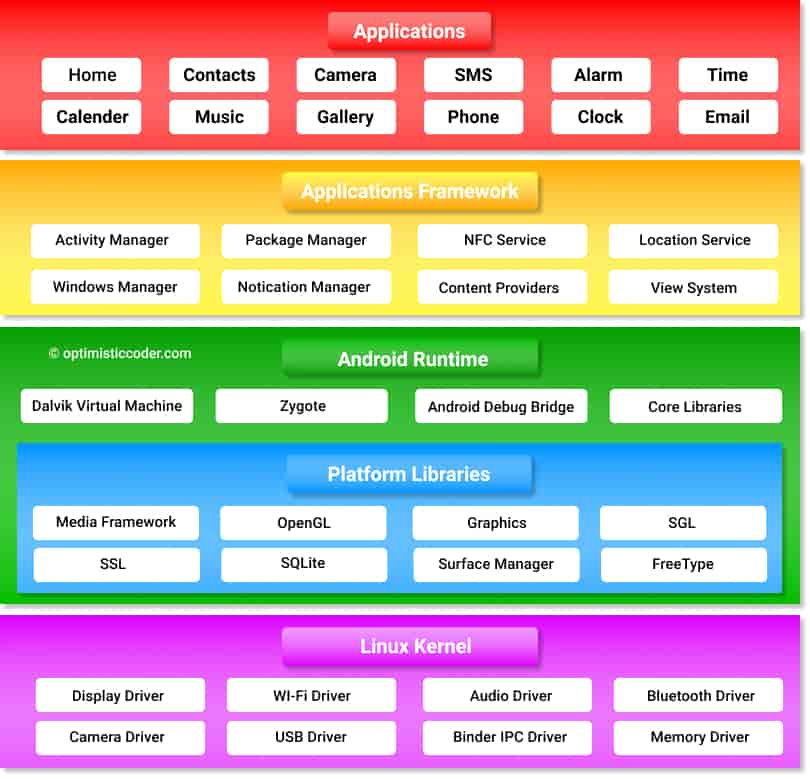
\includegraphics[width=0.8\textwidth]{./image/architecture.jpg}
  \end{center}
  \caption[android architecture]{android architecture}
  \label{fig:walrus}
  \end{figure}

\begin{enumerate}
    \item ชั้นแอพพลิเคชัน(Application) ชั้นนี้เป็นชั้นบนสุดของโครงสร้าง Android ซึ่งเป็นส่วน ของแอพพลิเคชันที่พัฒนาขึ้นมาใช้งาน เช่น แอพพลิเคชันรับส่งอีเมลล์ แอพพลิเคชันโทรศัพท์(Phone Dial) แอพพลิ-
    เคชันเว็บบราวเซอร์(Web Browser) เป็นต้น ทั้งนี้โปรแกรมในชั้น แอพพลิเคชันนั้นจะอยู่ ในรูปแบบของ
    ไฟล์.apk ซึ่งโดยทั่วไปแล้วจะอยู่ในไดเร็คทอรี่ data/app ของ โทรศัพท์
    
    \item ชั้นแอพพลิเคชันเฟรมเวิร์ค (Application Framework) โดยปกติแล้วนักพัฒนาสามารถ เรียกใช้
    งาน Android ผ่าน API (Application Programming Interface) ได้ ซึ่ง Android ได้ออกแบบ ไว้
    เพื่อลดความซ้า ซ้อนในการใช้งานซ้า ของ Application Component
    \item ชั้นไลบรารี(Library) แอนดรอยด์ได้รวบรวมกลุ่มของไลบรารีต่างๆ ที่สาคัญและมีความ จา เป็นต่อ
    การพัฒนาโปรแกรมเอาไว้มากมา ซึ่งถูกเขียนไว้ด้วยภาษา C และ C++

    \item ชั้นลีนุกซ์เคอร์เนล (Linux Kernel) ระบบ Android อยู่บนพื้นฐานของระบบปฏิบัติการ Linux
    โดยชั้น Linux Kernel นั้นมีฟั งก์ชันการทา งานหลายๆส่วน ซึ่งแต่ละส่วนถูกพัฒนาขึ้นด้วย ภาษา C เช่น
    การจัดการหน่วยความจา (Memory Management) การจัดการโพรเซส (Process Management) การ
    เชื่อมต่อเครือข่าย(Networking) และฟั งก์ชันการทางานส่วนอื่นที่เกี่ยวข้องกับ ระบบ ปฏิบัติการ ทั้งนี้นัก
    พัฒนาจะไม่มีสิทธ์ิ
    เข้าถึงส่วนนี้ได้โดยตรง ซึ่งนักพัฒนาสามารถเข้าถึง ระบบปฏิบัติ การ Linux ได้จากชุดคา
    สั่ง Command Prompt เช่น adb shell ซึ่งจะสามารถใช้ เครื่องมือต่างๆ ได้ เช่น การเข้าดูระบบไฟล์(File
    System) โพรเซสการคัดลอกไฟล์(Copy File) เป็นต้น
    
\end{enumerate}
\section{Development tools and technology}
\subsection{Firebase}
Firebase \cite{firebase} คือ Platform ที่รวบรวมเครื่องมือต่าง ๆ สําหรับการจัดการในส่วนของ Backend หรือ
Server side ซึ่งทําให้สามารถ Build Mobile Application ได้อย่างมีประสิทธิภาพ และยังลดเวลาและ
ค่าใช้จ่ายของการทํา Server side หรือการวิเคราะห์ข้อมูลให้อีกด้วย โดยมีทั้งเครื่องมือที่ฟรี และเครื่องมีที่
มีค่าใช้จ่าย (สําหรับการ Scale)

\subsubsection{ผลิตภัณฑ์ต่าง ๆ ของ Firebase}
Firebase มีผลิตภัณฑ์ทั้งหมดถึง 18 อย่างและแบ่งออกเป็น 3 หมวดหมู่ ดังนี้

\subsubsection{Build better apps}
มีทั้งหมด 7 ผลิตภัณฑ์ ได้แก่
\begin{enumerate}
  \item Realtime Database คือบริการฐานข้อมูล NoSQL ใช้วิธีการเก็บข้อมูลเป็น JSON Tree
  ขนาดใหญ่ และสามารถ Sync สถานะข้าม Client ได้แบบ Realtime กล่าวคือ หากเชื่อมต่อ Database
  เดียวกัน 2 ที่ เมื่อใดที่ที่นึงมีการอัพเดตข้อมูล อีกที่นึงก็จะมีการอัพเดตข้อมูลให้เหมือนกันโดยอัตโนมัติ และ
  สามารถทํางานแบบ Offline ได้บนแอป Android และ iOS
  
  \item Authentication คือบริการตรวจสอบผู้ใช้ โดยสามารถตรวจสอบได้หลายวิธี เช่น Email/Password, เบอร์โทรศัพท์, บัญชีGoogle, Facebook, Twitter, Github เป็นต้น มีฐานข้อมูลเป็นของตัวเอง
  ไม่ต้องสร้างใหม่หรือออกแบบวิธีการเก็บซึ่ง สามารถดูได้ว่าสมัครด้วยวิธีไหน สมัครเมื่อไหร่ และเข้าใช้ระบบ
  ครั้งล่าสุดเมื่อไหร่
  
  \item  Hosting คือบริการฝากไฟล์static เช่น HTML, CSS, JS, JPG(ไม่รองรับ PHP ซึ่งเป็น
  Dynamic) เพื่อให้คนอื่น ๆ เข้าใช้งานเว็บของเราได้ มักนิยมใช้ในการฝากไฟล์ที่ได้จากการ Build ของ
  JavaScript Framework ต่าง ๆ เช่น Angular, React, Vue สังเกตว่าจะได้ไฟล์HTML, CSS, JS
  ต่าง ๆ ตามที่ได้บอกไว้ข้างต้น หรือจะเป็นไฟล์ที่เขียนเองก็ได้ ไม่จําเป็นต้องใช้Framework ก็ได้เหมือนกัน
  อีกทั้งมีCDN และ SSL มาด้วยแบบฟรี ๆ เพื่อให้ผู้ใช้ของคุณได้รับประสบการณ์การใช้งานที่ปลอดภัยเชื่อถือได้และไม่มีความล่าช้าแม้ว่าจะอยู่ที่ไหนก็ตาม ทุกเว็บมีDomain Name ของ Firebase ให้อัตโนมัติ แต่
  เปลี่ยนมาใช้ของตัวเองได้

  \item Cloud Functions คือบริการสําหรับ Deploy Function ที่พัฒนาด้วย JavaScript หรือ
TypeScript เพื่อทํางานตาม Tigger (คล้าย ๆ event) ที่เกิดขึ้นบน Firebase เช่น ถ้า Database ถูก
เขียน (Realtime Database Triggers) ให้Function เราส่ง Notification แจ้งไปบอกเราด้วย หรือ มี
การเรียนมาที่ HTTP Endpoint (HTTP Triggers) ให้Function เราคืนค่า HTML กลับไป (ใช้ทํา
REST API) หรือ ถ้าแอปมีปัญหา (Crashlytics Triggers) ให้ส่งข้อความแจ้งเตือนไปที่ Slack

  \item Cloud Storage คือบริการเก็บไฟล์รูปภาพ, ไฟล์เสียง, วิดีโอ เพื่อใช้บน Application เช่น
  รูปภาพประจําตัวสมาชิก, วิดิโอสอนการใช้งานโปรแกรม เป็นต้น
  \item Cloud Firestore (Beta) คือ Realtime Database รุ่นใหม่มาพร้อมการค้นหาและการปรับ
  ขนาดอัตโนมัติที่มีประสิทธิภาพมากขึ้น ปรับปรุงวิธีการเก็บข้อมูลใหม่เป็น Collections และสามารถทํางาน
  แบบ Offline บน Web ได้อีกด้วย (จากเดิมทําได้แค่บน Android และ iOS)
  \item ML Kit (Beta) คือ Machine Learning SDK ที่ช่วยให้แอปมือถือสามารถใช้ความสามารถ
  ของ ML ได้ง่ายยิ่งขึ้น สามารถทํางานได้ทั้งแบบ Online และ Offline
\end{enumerate}

\subsubsection{Improve app quality}
มีทั้งหมด 3 ผลิตภัณฑ์ ได้แก่
\begin{enumerate}
  \item Crashlytics คือบริการตรวจจับและแจ้งเตือนหากแอปเราเกิดอาการ Crash ขึ้นแบบ Realtime
  เพื่อให้แอปเราเสถียรอยู่เสมอ โดยจะทําการแจ้งให้ทราบถึงข้อผิดพลาดและผลกระทบ ผ่านทาง E-mail และ
  Firebase Console (ใช้Cloud Functions เพื่อส่งไปที่อื่นด้วยได้ เช่น slack) เพื่อการแก้ปัญหาที่รวดเร็ว
  และตรงจุด
  
  \item Performance Monitoring คือบริการตรวจสอบคุณภาพของแอป เพื่อให้แอปของเราตอบสนอง
  ได้เร็วอยู่เสมอ โดยสามารถตรวจสอบเวลาและรายละเอียดการทํางานต่าง ๆ เช่น เวลาที่ใช้ในการเปิ ดแอป ,
  เวลาที่ใช้การเปลี่ยนหน้า UI, เวลาที่ใช้ในการโหลด API, ขนาดข้อมูลที่ Download/Upload, จํานวน
  API ที่สําเร็จหรือล้มเหลว เป็นต้น
  
  \item  Test Lab คือบริการทดสอบแอปบนฮาร์ดแวร์จริง ๆ เพื่อให้มั่นใจว่าแอปของเราสามารถรองรับ
  ฮาร์ดแวร์ที่เราต้องการได้จริง ๆ โดยสามารถระบุรุ่นและเวอร์ชันที่ต้องการได้ แล้วระบุรูปแบบการทดสอบต่าง
  ๆ เพื่อทดสอบและรายงานผลกลับมา ไม่ต้องซื้อโทรศัพท์เอง (สมมุติว่าจริงจังเรื่องการรองรับทุกอุปกรณ์มาก)
  ซึ่งเป็นเรื่องยากด้วยหากจะซื้อทุกรุ่นที่คนนิยมใช้ในตลาด ไหนจะต่อสาย จะนั่งทดสอบทีละเครื่องอีก ใช้ตัวนี้
  จบ หมดปัญหา
\end{enumerate}

\subsubsection{Grow your business}
มีทั้งหมด 8 ผลิตภัณฑ์ ได้แก่ 
\begin{enumerate}
  \item  In-App Messaging คือบริการแสดงข้อความ pop-up ภายในแอป
  ของเรา เช่น โฆษณา (เจอประจําเลย), การแจ้งเตือน, ข่าวสาร เป็นต้น

  \item  Google Analytics คือบริการแสดงข้อมูลสถิติต่าง ๆ ของแอป เช่น ใช้ด้วยระบบปฏิบัติการอะไร
  จํานวนเท่าไหร่, มีผู้ใช้งาน ณ ปั จจุบันกี่คน, ใช้งานส่วนไหนบ้าง เป็นต้น เพื่อวิเคราะห์กลุ่มเป้ าหมาย หรือรับ
  ทราบพฤติกรรมของผู้ใช้งานต่าง ๆ
  
  \item Predictions คือบริการวิเคราะห์ข้อมูลการใช้งานแอป ช่วยให้เรารู้ว่าผู้ใช้ใช้งานส่วนใดบ้างในแอป
  ช่วยให้เรารู้ว่าส่วนใดตอบสนองได้ดี ส่วนใดควรปรับปรุง หรืออาจต้องการที่จะหยั่งรู้พฤติกรรมในอนาคตของ
  ผู้ใช้งานแอปของคุณ เพื่อวางแผนกลยุทธ์ทั้งรุกและรับ รวมทั้งสร้างประสบการณ์ที่น่าประทับใจให้กับผู้ใช้ของ
  เรา
  \item Cloud Messaging คือบริการส่งการแจ้งเตือนไปยังมือถือหรือเว็บของเรา เพื่อแจ้งข้อความไป
  ยังผู้ใช้ของเราแม้ว่าจะปิ ดแอปไปแล้วก็ตาม ถ้าใครใช้Smartphone อยู่(น่าจะทุกคนแหละ ที่กําลังอ่านบทความนี้อยู่) จะคุ้นเคยกันเป็นอย่างดี เช่น การแจ้งเตือนจาก facebook, line, instagram ต่าง ๆ เป็นต้น
  
  \item    Remote Config คือความสามารถที่จะเปลี่ยนลักษณะการทํางานและลักษณะที่ปรากฏของแอป
  ของคุณได้ทันทีจากหน้าเว็บ Firebase โดยไม่ต้องรอการอนุมัติจาก App Store เช่น การเปลี่ยนรูปแบบ
  ตามเทศกาล, เปลี่ยนภาษาตามผู้ใช้งาน เป็นต้น
  \item   Dynamic Links คือลิ้งค์เชื่อมโยงไปยังแอปมือถือ ใช้สําหรับแสดงบนหน้าเว็บเพื่อให้ผู้ใช้งานติด
  ตั้งแอปมือถือผ่านลิ้งค์ลิ้งค์นี้ อีกทั้งยังสามารถแนบข้อมูลต่าง ๆ ของผู้ใช้ที่อยู่บนเว็บมาด้วยได้  
  \item    App Indexing คือการปรับแต่งแอปของเราให้แสดงผลข้อมูลภายในแอปบน Google Search
  ได้(เรียกการทํา SEO แบบ Mobile App ก็คงไม่ผิด) เช่น ค้นชื่อร้านอาหารแล้วปรากฏแอปวงในขึ้นมาให้
  ดูรายละเอียดและรีวิว เป็นต้น
  
  \item   A/B Testing (Beta) คือความสามารถในการแสดงผลแอปหลายรูปแบบเพื่อทดสอบการแสดง
  ผลหรือการทํางาน ว่าสิ่งไหนจะมอบประสบการณ์การใช้งานที่ดีกว่าให้แก่ผู้ใช้งาน เช่น การวางป่ ุมกดแบบ
  ไหนที่ผู้ใช้งานใช้สะดวก สมมุติว่ามีผู้ใช้งาน 100 คน อาจจะมี50 คนได้ป่ ุมที่อยู่มุมบน อีก 50 คนได้ป่ ุมอยู่
  มุมล่าง หากว่ามีการใช้งานแบบไหนมากกว่ากันก็อาจจะสรุปผลและเลือกใช้แบบนั้นกับทุกคนในท้ายที่สุด

\end{enumerate}

\subsection{Android Studio}
Android Studio \cite{android_studio} เป็น IDE Tool จาก Google ไว้พัฒนา Android สําหรับ Android Studio
เป็น IDE Tools ล่าสุดจาก Google ไว้พัฒนาโปรแกรม Android โดยเฉพาะ โดยพัฒนาจากแนวคิดพื้น
ฐานมาจาก InteliJ IDEA คล้าย ๆ กับการทํางานของ Eclipse และ Android ADT Plugin โดยวัตถุ-
ประสงค์ของ Android Studio คือต้องการพัฒนาเครื่องมือ IDE ที่สามารถพัฒนา App บน Android ให้
มีประสิทธิภาพมากขึ้น ทั้งด้านการออกแบบ GUI ที่ช่วยให้สามารถ Preview ตัว App มุมมองที่แตกต่างกัน
บน Smart Phone แต่ล่ะรุ่น สามารถแสดงผลบางอย่างได้ทันทีโดนไม่ต้องทําการรัน App บน Emulator
รวมทั้งยังแก้ไขปรับปรุงในเรื่องของความเร็วของ Emulator ที่ยังเจอปัญหากันอยู่ในปั จจุบัน

\subsection{JSON (Java Script Object Notation)}
JSON \cite{json} ย่อมาจากคําว่า Java Script Object Notation เป็นฟอร์แมตสาหรับการแลกเปลี่ยนข้อมูล
ที่มีขนาดเล็ก ซึ่งสามารถทําความเข้าใจได้ง่าย และสามารถถูกสร้างและอ่านโดยเครื่องได้ง่าย ซึ่ง JSON ถูก
กําหนดให้อยู่ภายใต้ภาษา Java Script (Java Script Programming Language,Standard ECMA262
3rd Edition - December 1999.) ที่มีรูปแบบข้อมูลตัวอักษรที่มีความอิสระอย่างสมบูรณ์ แต่จะ มีหลัก
การเขียนคุ้นเคยกับนักเขียนโปรแกรมภาษาต่างๆ เช่น ภาษา C, C++, Java, Javascript, Perl, Phython
และอื่นๆ คุณสมบัติเหล่านี้ทําให้JSON เป็นภาษาในการแลกเปลี่ยนข้อมูลที่มีความ สมบูรณ์แบบ ประเภท
ของ JSON
\begin{enumerate}
  \item  Client-server architecture: Client ไม่จําเป็นต้องรู้อะไรเกี่ยวกับ Business logic ภายใน ไม่มี
  หน้าที่เกี่ยวกับการจัดเก็บข้อมูล ส่วน Server มีหน้าที่เก็บ Resource และไม่จําเป็นต้องรู้อะไรเกี่ยว
  กับ UI Frontend หรือสถานะของผู้เรียก
  

  \item  Number: ตัวเลขเท่านั้น
  
  \item String: Unicode ใช้เครื่องหมาย double-quote (“) เป็นตัวบ่งบอก และสามารถใช้backslash
  syntax ได้
  
  \item Boolean: True or False
  \item    Array: ชุดข้อมูล ซึ่งจะเป็นชนิดใดก็ได้ ใช้สัญลักษณ์square bracket [var1,var2] เป็นตัวแสดง
  และคั้นด้วย comma แต่ะลค่าใน array
  \item  Object: ชุดข้อมูลที่เป็นคู่Key-Value แบบ strings [key1:value1, key2:value2] ใช้comma
  เป็นตัวแบ่งแต่ละคู่ และใช้colon เป็นตัวแบ่งระหว่าง key และ value
  \item    Null: ค่าว่าง
\end{enumerate}

\subsection{NoSQL Databases}
ฐานข้อมูล NoSQL \cite{nosql_is}  สร้างตามวัตถุประสงค์สําหรับโมเดลข้อมูลแบบเฉพาะเจาะจงและมีแบบแผนที่
ยืดหยุ่นสําหรับการสร้างแอปพลิเคชันอันทันสมัย ฐานข้อมูล NoSQL เป็นที่รู้จักกันดีในด้านความง่ายในการ
พัฒนา การทํางาน และประสิทธิภาพตามขนาดที่ต้องการ หน้านี้ประกอบด้วยทรัพยากรเพื่อช่วยให้คุณเข้าใจ
ฐานข้อมูล NoSQL และเริ่มต้นใช้งาน
\subsection{Android SDK}
Android Software Development Kit (Android SDK)\cite{sdk_tool}  เปรียบเสมือน Library ที่ใช้ใน
การพัฒนา Application สําหรับ Android เนื่องจากตัว Android มีหลายเวอร์ชั่นและแต่ละเวอร์ชั่นมี
Feature, GUI ที่ไม่เหมือนกันทําให้เกิด Android SDK ออกมาหลายเวอร์ชั่นให้เลือกใช้งาน

\subsection{JDK (Java Development Kit)}
Java Development Kit หรือ JDK \cite{android_studio} คือชุดของเครื่องมือที่ใช้ในการพัฒนาโปรแกรม JAVA ของ
บริษัทซัน ไมโครซิสเต็มส์ นักกพัฒนาโปรแกรมโดยใช้ภาษา Java อย่างเช่น Java Compiler, Java Debugger, Java Doc และ Java Interpreter หรือ Java VM จะต้องติดตั้ง JDK นี้ ไม่ งั้นจะไม่สามารถ
Compile และ Run java ได้ เวอร์ชันปั จจุบันของ JDK คือเวอร์ชั่น 7 ประกอบไป ด้วยโปรแกรมต่างๆ
อาทิเช่น โปรแกรม คอมไพเลอร์(javac.exe) โปรแกรมอินเตอร์พรีตเตอร์(java.exe) โปรแกรมดีบักเกอร์
แต่จะไม่มีโปรแกรม อีดิเตอร์
\begin{enumerate}
  \item  Java SE (Standard Edition) สําหรับพัฒนาโปรแกรมบนคอมพิวเตอร์ตั้งโต๊ะทั่วไป
  
  \item  Java ME (Micro Edition) สําหรับพัฒนาโปรแกรมบนอุปกรณ์พกพา เช่น โทรศัพท์มือถือหรือพี
  ดีเอ ส่วนมากใช้เขียนโปรแกรมเกม
  
  \item Java EE (Enterprise Edition) สําหรับพัฒนาโปรแกรมในองค์กรใหญ่ๆ หรือมี ขอบเขตของโครงการกว้างมาก
\end{enumerate}
\subsection{SDK Platform (Software Development Kit )}
SDK  ซึ่งย่อมาจาก Software Development Kit \cite{sdk_tool} คือเครื่องมือที่เอาไว้สําหรับพัฒนาโปรแกรมหรือ
แอพพิเคชั่นบนระบบ Android OS ซึ่งทาง Google พัฒนาออกมาเพื่อแจกจ่ายให้นักพัฒนาแอพพลิเคชั่น
หรือผู้สนใจทั่วไปดาวน์โหลดไปใช้กันโดยไม่มีค่าใช้จ่าย และนี่ก็เป็นหนึ่งในปั จจัยที่ทําให้แอพพลิเคชั่นบนแอน
ดรอยด์นั้นเพิ่มขึ้น อย่างรวดเร็ว ซึ่งในชุด SDK นั้นจะมีโปรแกรมและไลบรารี่ต่างๆ ที่จําเป็นต่อการพัฒนา
แอพพลิเคชั่นบนแอนดรอยด์ อย่างเช่น Emulator ซึ่งทําให้ผู้ใช้สามารถสร้างแอพพลิเคชั่นและนํามาทดลอง
รันบนตัวอีมูเลเตอร์ ก่อน โดยมีสภาวะแวดล้อมเหมือนมือถือที่รันระบบปฏิบัติการแอนดรอยด์จริงๆ
\subsection{AVD (Android Visual Device)}
ADV ย่อมาจาก android virtual device \cite{adv_is}  คือ การจำลอง หรือ Emulator เครื่องโทรศัพท์มือถือระบบปฎิบัติการแอนดรอยด์ บนเครื่องคอมพิวเตอร เพื่อ เอาไว้ทดสอบ โปรแกรม หรือ โค้ด โปรแกรมที่ได้เขียนขึ้น

ข้อดีของ ADV

AVD นั้น เป็น Emulator ที่เพิ่มความสะดวกสบายในการพัฒนา Application สำหรับ Android โดยหลังจากที่ผู้พัฒนาเขียน App เสร็จแล้ว ก็สามารถส่ง App ไปลองรันบน คอมพิวเตอร์ ที่ได้ทำให้เป็น Emulator ดูได้เลย แต่สำหรับผู้ใช้งานทั่วไปนั้น เราก็สามารถนำเจ้าตัว App ตัวนี้ มาลองใช้เล่นๆเหมือนเป็น Android Device บนเครื่องนึงบนคอมพิวเตอร์ที่ได้ทำให้เป็น Emulator ได้
% \begin{equation}\label{eq:dielectric}
% k_1=\frac{\omega}{c({1/\varepsilon_m + 1/\varepsilon_i})^{1/2}}=k_2=\frac{\omega
% \sin(\theta)\varepsilon_\mathit{air}^{1/2}}{c}
% \end{equation}

% \noindent
% where $\omega$ is the frequency of the plasmon, $c$ is the speed of
% light, $\varepsilon_m$ is the dielectric constant of the metal,
% $\varepsilon_i$ is the dielectric constant of neighboring insulator,
% and $\varepsilon_\mathit{air}$ is the dielectric constant of air.

% \section{About using figures in your report}

% % define a command that produces some filler text, the lorem ipsum.
% \newcommand{\loremipsum}{
%   \textit{Lorem ipsum dolor sit amet, consectetur adipisicing elit, sed do
%   eiusmod tempor incididunt ut labore et dolore magna aliqua. Ut enim ad
%   minim veniam, quis nostrud exercitation ullamco laboris nisi ut
%   aliquip ex ea commodo consequat. Duis aute irure dolor in
%   reprehenderit in voluptate velit esse cillum dolore eu fugiat nulla
%   pariatur. Excepteur sint occaecat cupidatat non proident, sunt in
%   culpa qui officia deserunt mollit anim id est laborum.}\par}

% \begin{figure}
%   \centering

%   \fbox{
%      \parbox{.6\textwidth}{\loremipsum}
%   }

%   % To include an image in the figure, say myimage.pdf, you could use
%   % the following code. Look up the documentation for the package
%   % graphicx for more information.
%   % \includegraphics[width=\textwidth]{myimage}

%   \caption[Sample figure]{This figure is a sample containing \gls{lorem ipsum},
%   showing you how you can include figures and glossary in your report.
%   You can specify a shorter caption that will appear in the List of Figures.}
%   \label{fig:sample-figure}
% \end{figure}

% Using \verb.\label. and \verb.\ref. commands allows us to refer to
% figures easily. If we can refer to Figures
% \ref{fig:walrus} and \ref{fig:sample-figure} by name in the {\LaTeX}
% source code, then we will not need to update the code that refers to it
% even if the placement or ordering of the figures changes.

% \loremipsum\loremipsum

% % This code demonstrates how to get a landscape table or figure. It
% % uses the package lscape to turn everything but the page number into
% % landscape orientation. Everything should be included within an
% % \afterpage{ .... } to avoid causing a page break too early.
% \afterpage{
%   \begin{landscape}
%   \begin{table}
%     \caption{Sample landscape table}
%     \label{tab:sample-table}

%     \centering

%     \begin{tabular}{c||c|c}
%         Year & A & B \\
%         \hline\hline
%         1989 & 12 & 23 \\
%         1990 & 4 & 9 \\
%         1991 & 3 & 6 \\
%     \end{tabular}
%   \end{table}
%   \end{landscape}
% }

% \loremipsum\loremipsum\loremipsum

% \section{Overfull hbox}

% When the \verb.semifinal. option is passed to the \verb.cpecmu. document class,
% any line that is longer than the line width, i.e., an overfull hbox, will be
% highlighted with a black solid rule:
% \begin{center}
% \begin{minipage}{2em}
% juxtaposition
% \end{minipage}
% \end{center}

\section{\ifenglish%
\ifcpe CPE \else ISNE \fi knowledge used, applied, or integrated in this project
\else%
ความรู้ตามหลักสูตรซึ่งถูกนำมาใช้หรือบูรณาการในโครงงาน
\fi
}

ความรู้ตามหลักสูตรที่นํามาใช้ในการพัฒนาแอปพลิเคชันได้แก่ ได้แก่ ด้นําความรู้จากวิชา Data Structure, Database, OOP Programming และ Algorithm มาใช้ในการออกแบบ Database ของโครงการ นอกจากนี้ยังใช้ความรู้จาก Software Project Management มาช่วยในการวางแผนงานและการ
วางแผนการจัดการในด้านต่างๆ และIntroduction to Human-Computer Interaction มาช่วยในการ
ออกแบบ UX/UI

\section{\ifenglish%
Extracurricular knowledge used, applied, or integrated in this project
\else%
ความรู้นอกหลักสูตรซึ่งถูกนำมาใช้หรือบูรณาการในโครงงาน
\fi
}

ความรู้นอกหลักสูตรที่นํามาใช้ในการพัฒนาแอปพลิเคชันได้แก่Android studio การใช้Emulator,โครงสร้าง
Mobile Application และการประยุกต์ใช้งาน service ต่างๆจาก Firebase

\chapter{\ifproject%
\ifenglish Project Structure and Methodology\else โครงสร้างและขั้นตอนการทำงาน\fi
\else%
\ifenglish Project Structure\else โครงสร้างของโครงงาน\fi
\fi
}

ในบทนี้จะกล่าวถึงหลักการ และการออกแบบระบบ

\makeatletter

% \renewcommand\section{\@startsection {section}{1}{\z@}%
%                                    {13.5ex \@plus -1ex \@minus -.2ex}%
%                                    {2.3ex \@plus.2ex}%
%                                    {\normalfont\large\bfseries}}

\makeatother
%\vspace{2ex}
% \titleformat{\section}{\normalfont\bfseries}{\thesection}{1em}{}
% \titlespacing*{\section}{0pt}{10ex}{0pt}

\section{ขั้นตอนการดําเนินงาน}

\subsection{ขั้นตอนการเก็บ requirements}
\subsubsection{สำหรวจปัญหาจากการสอบถาม}
การสําหรวจจากการสอบถามของตัวแทนนักศึกษา 10 คน โดยมีวัตถุประสงค์เพื่อแก้ปัญหาต่างๆในการใช้
ชีวิตในมหาวิทยาลัย โดยเน้นไปที่การช่วยเหลือนักศึกษาใหม่ที่เป็นช่วงในการปรับตัวเข้ากับสังคมในมหาวิทยาลัย

\subsubsection{วิเคราะห์ปัญหา}
สามารถสรุปได้เป็นประเด็นดังนี้
\begin{enumerate}
  \item การที่เราอยากรู้ถึงวิธีการแก้ปัญหาที่เราเผชิญอยู่นั้นการค้นหาข้อมูลจากอินเทอร์เน็ต โดยส่วนมากการ
  ค้นหาข้อมูลที่มีลักษณะ เป็นประสบการณ์จากคนที่เคยแก้ปัญหาเรื่องนั้นมาก่อน บางครั้งการค้นหา
  ข้อมูลลักษณะนี้มักจะหาข้อมูลได้ยาก การใช้คําในการค้นหา ข้อมูลกระจายไปในที่ต่างๆหลากหลาย
  เวปไชต์ยิ่งต้องใช้เวลาในการเพิ่มไปอีก นอกจากนี้ยิ่งเป็นเรื่องราวเฉพาะพื้นที่ทําให้ข้อมูลยิ่งหายากมาก
  ขึ้น
  \item การขอคําปรึกษาจากผู้ที่เรารู้จักนั้น บางครั้งอาจจะได้คําตอบที่ไม่ตรงกับที่คาดหวังอาจเนื่องมาจากผู้
  ที่เราขอความช่วยเหลื่อไม่มีความรู้หรือประสบการในเรื่องนั้น
  
  \item การสอบคําถามนั้นบางครั้งผู้ถามอาจจะเกิดความเขินอายในการที่จะถามในเรื่องนั้นออกไป ทําให้ไม่
  ความความกล้าในการขอความช่วยเหลือ
  
  \item ในกรณีของนักศึกษาใหม่การหาหอพัก สวัสดิการช่วยเหลือของมหาลัยไม่ค่อยเป็นที่พูดถึงในโชเชียลมา
  กนัก บางครั้งอาจได้รับข้อมูลที่ผิดจากคนที่ไม่มีประสบการณ์และไม่รู้จริง
\end{enumerate}

\subsubsection{สรุปปัญหาหาแนวทางแก้ไขและออกแบบ}
\begin{enumerate}
  \item ออกแบบแอปพลิเคชันที่สามารถเป็นสื่อกลางในการรวบรวมประสบการณ์ต่างๆจากการรีวิว มีการแบ่ง
  เป็นหมวดหมู่สามารถเข้าถึงได้ง่าย ซึ่งตัวแอปพลิเคชันจะมีวัตถุประสงค์ในการช่วยเหลือนักศึกษามหาวิทยาลัยเชียงใหม่ทําให้มีลักษณะของการรวมคนเฉพาะพื้นที
  
  \item ในเรื่องของความน่าเชื่อถือของการีวิวสามารถดูได้จากคะแนนการรีวิวยิ่งคะแนนมาก ความน่าเชื่อถือ
  ยิ่งมาก
  \item สามารถถามคําถามเพื่อหาคนที่เราสามารถขอคําปรึกษาจากผู้ที่รู้และมีประสบการณ์ในเรื่องนั้นๆ
  \item สามารถปิดบังตัวตนเพื่อเพิ่มความกล้าในการขอความช่วยเหลือ
\end{enumerate}

\subsubsection{ขั้นตอนการออกแบบระบบ}
\begin{enumerate}
  \item ออกแบบ Use case diagram
  \item เลือกเทคโนโลยีและเครื่องมือที่จะใช้
  
  \item  ออกแบบ UI ใน Figma โดยมีพื้นฐานการออกแบบมาจากการใช้งานแอปพลิชันโซเชียลมีเดียทั่วไป
  
\end{enumerate}
\section{โครงสร้างของแอปพลิเคชัน}
\subsection{Use case diagram}
แสดงให้เห็นภาพรวมของการใช้งานระบบดังรูปที่ 3.1 จาก requirement เราสามารถระบุUser คือกลุ่ม
บุคคลที่ใช้แอปพลิเคชันทั่วไป เมื่อเข้าสู่ระบบมาแล้วสามารถเข้าถึง Use case ต่างๆได้ดังนี้
\begin{enumerate}
  \item การรีวิว สามารถสร้างการีวิวเรื่องต่างๆ สามารถเข้ามาอ่านการรีวิว สามารถคอมเม้นและให้คะแนน
  การรีวิว
  \item กระดานตั้งกระทู้ถาม-ตอบ สามารถเข้าอ่าน ช่วยตอบข้อสงสังต่างๆผ่านการดานถามตอบปัญหาหรือ
  สร้างกระทู้ถามคําถามเองก็ได้
  \item  ระบบสนทนา สามารถเเชทเพื่อปรึกษาหารือกันได้

\end{enumerate}
\begin{figure}[ht]
  \begin{center}
    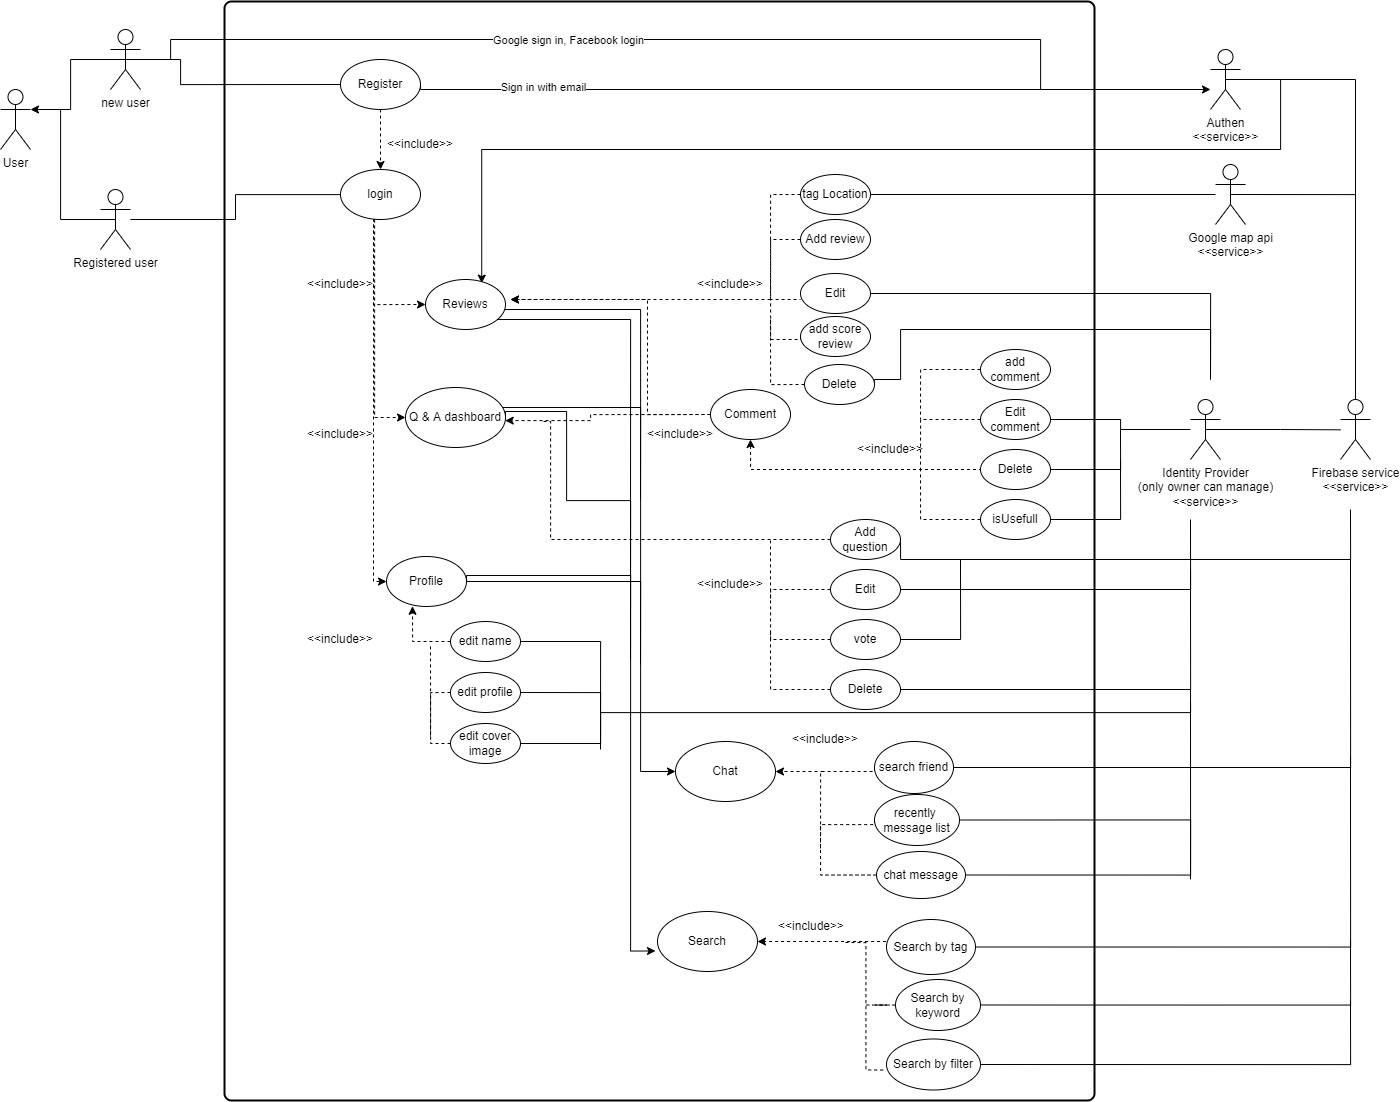
\includegraphics[width=1\textwidth]{./image/user-diagram.jpg}
  \end{center}
  \caption[Poem]{Use case diagram}
  \end{figure}

\subsection{System architecture}
สถาปัตยกรรมโครงสร้างของระบบในส่วนของการแสดงผลของ mobile application จะใช้java ในการเขียนแอพพลิเคชันและเชื่อมต่อ backend ด้วย firebase โดยบริการที่ใช้ของfirebaseได้แก่ Realtime Database
,Authentication และ Storage 

การลงชื่อเข้าใจสามารถลงชื่อผ่านแพลตฟอร์มอื่นได้ เช่น google(ผ่าน firebase Authentication) ,facebook(ผ่าน facebook api) ข้อมูลที่ใช้ในระบบจะถูกเก็บไว้ในฐานข้อมูล
บน firebase realtime ส่วนการเก็บข้อมูลของรูปภาพจะเก็บไว้ที่ firebase storage สามารถแท็ก location ที่อยู่บน google map  ดังรูปที่ 3.2  

\begin{figure}[ht]
  \begin{center}
    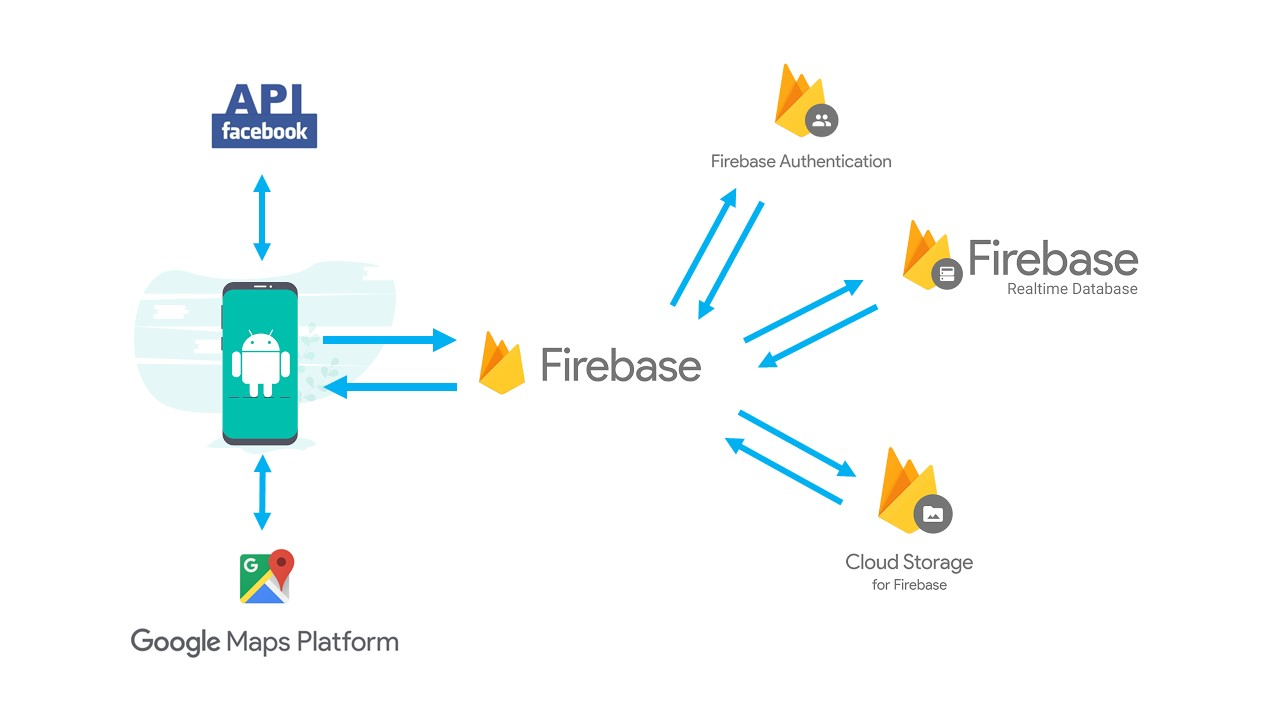
\includegraphics[width=0.9\textwidth]{./image/structure.jpg}
  \end{center}
  \caption[Poem]{System architecture}
  \end{figure}

\newpage
\subsection{Database schema}
 การเก็บข้อมูลในรูปแบบ NoSQL เก็บเป็น collections ต่างๆ ดังรูปที่ 3.3 
\begin{enumerate}
  \item Users จะเก็บข้อมูลของผู้ใช้
  \item Reviews จะเก็บข้อมูลของการรีวิว
  \item Rparticipation เก็บข้อมูลการมีส่วนร่วมกับ Reviews เช่น การให้คะแนนรีวิว
  \item QuestionAns จะเก็บข้อมูลของการกระดานถาม-ตอบ
  \item Qparticipation เก็บข้อมูลการมีส่วนร่วมกับ QuestionAns เช่น การกดถูกใจ
  \item MyLocation เก็บรายละเอียดของตำแหน่งที่ตั้ง
  \item Comments จะเก็บข้อมูลของคอมเมนต์
  \item MessageList จะเก็บข้อมูลของรายชื่อผู้รับ-ผู้ส่ง
  \item Chats จะเก็บข้อมูลรายละเอียดเนื้อหาการสนทนา
\end{enumerate}
\begin{figure}[ht]
  \begin{center}
    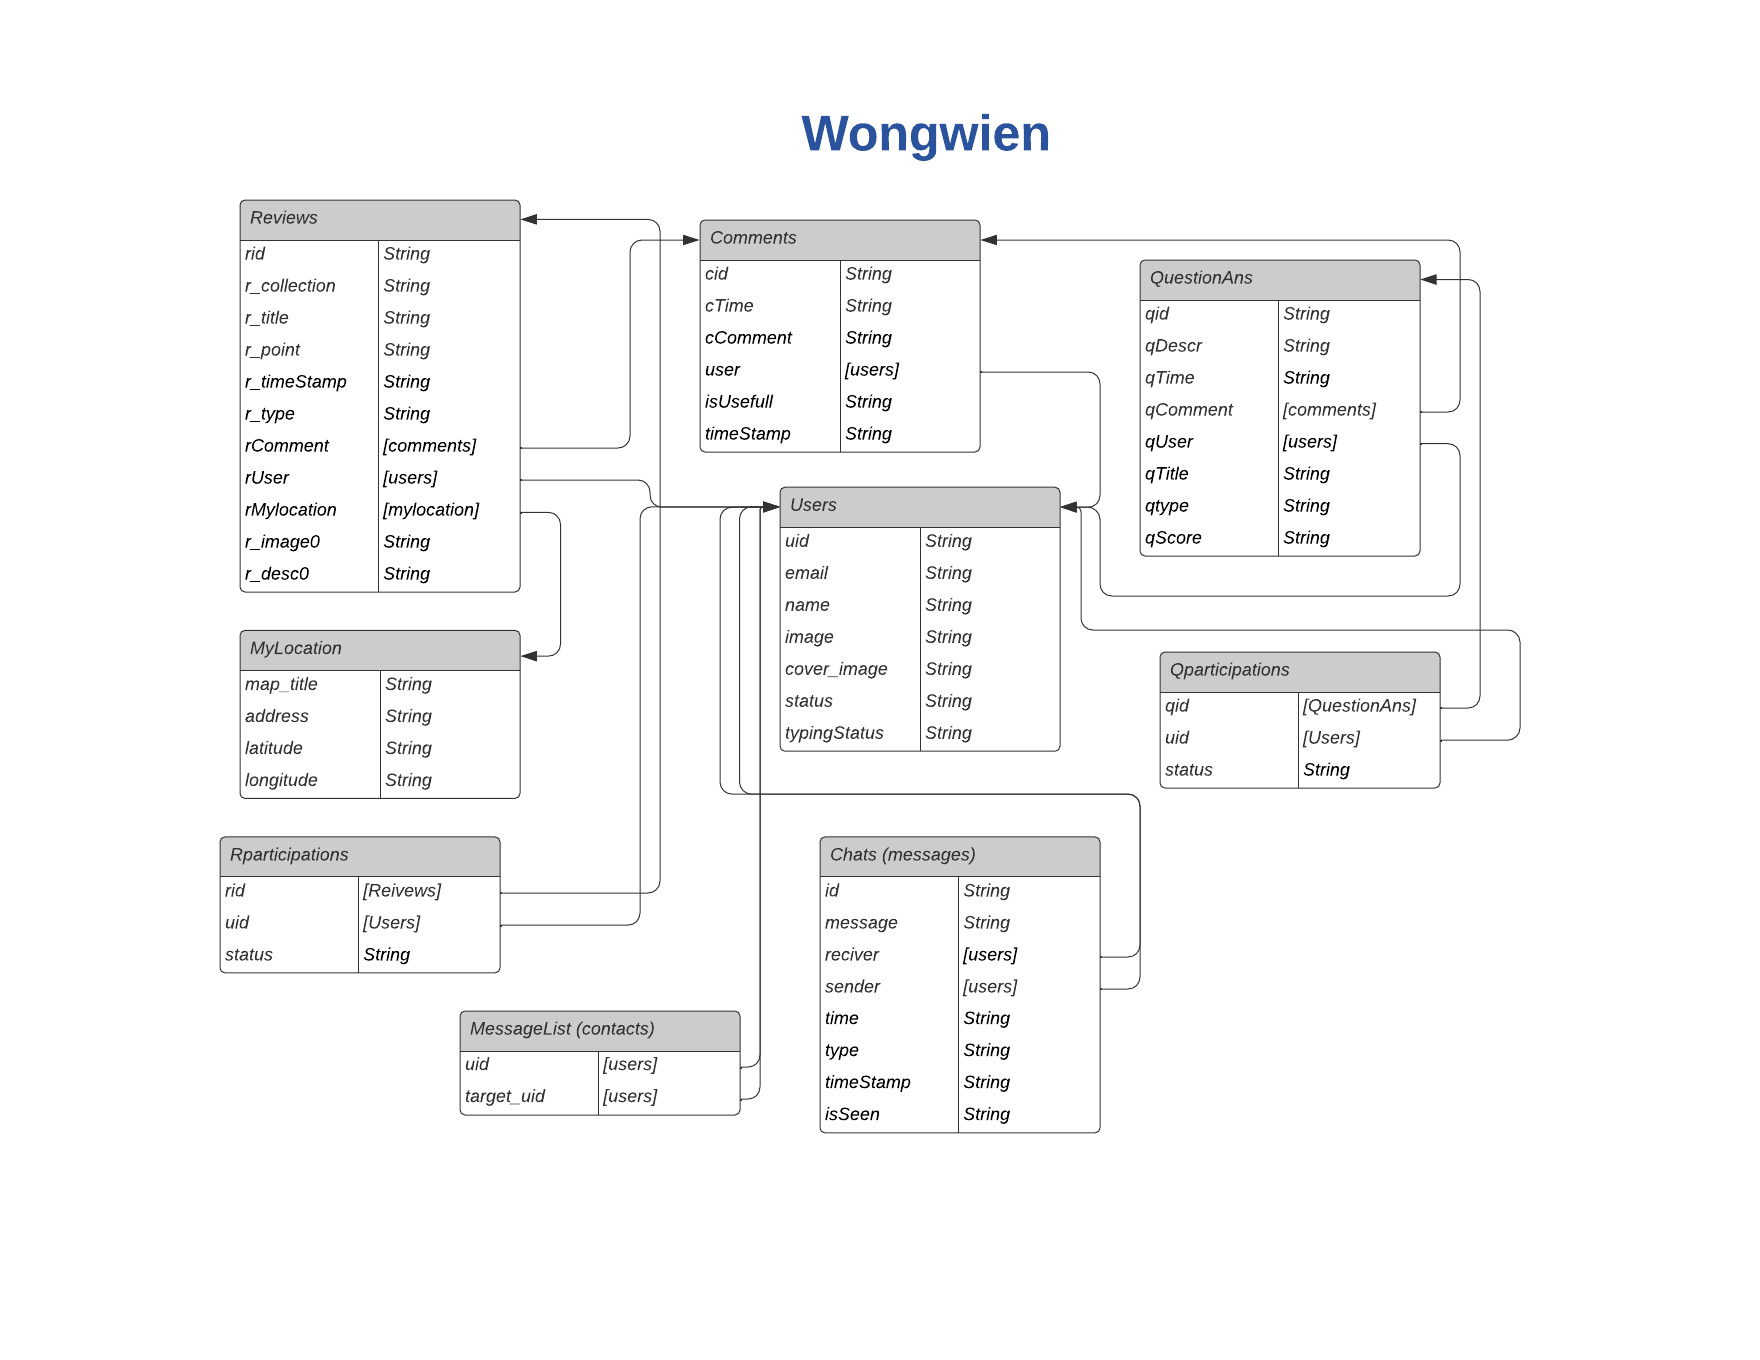
\includegraphics[width=1\textwidth]{./image/database.jpeg}
  \end{center}
  \caption[Poem]{System architecture}
  \end{figure}


\section{โครงสร้างของแอปพลิเคชัน}
\subsection{Use case diagram}


\chapter{\ifproject%
\ifenglish Experimentation and Results\else การทดลองและผลลัพธ์\fi
\else%
\ifenglish System Evaluation\else การประเมินระบบ\fi
\fi}

\quad \quad ในบทนี้จะทดสอบเกี่ยวกับการทำงานในฟังก์ชันหลักของแพลตฟอร์มว่าสามารถทำงานได้
หรือไม่ โดยมีการทดสอบการทำงานต่าง ๆ ดังนี้

\section{การทดสอบโดยการการยืนยันตัวตนผ่าน google}
\quad \quad การทดสอบโดยการการยืนยันตัวตนผ่าน google จะเรียกใช้ Firebase Authentication เข้ามาช่วยในการจัดการ
โดยการทดลองจะทำการเข้าสู่ระบบยืนยันตัวตนโดยผ่านบัญชี google ผลลัพธ์คือสามารถเข้าสู่ระบบได้สำเหร็จและสามารถดึงข้อมูลส่วนตัวมาได้
ดังรูป 4.1 
    \begin{figure}
    \begin{center}
      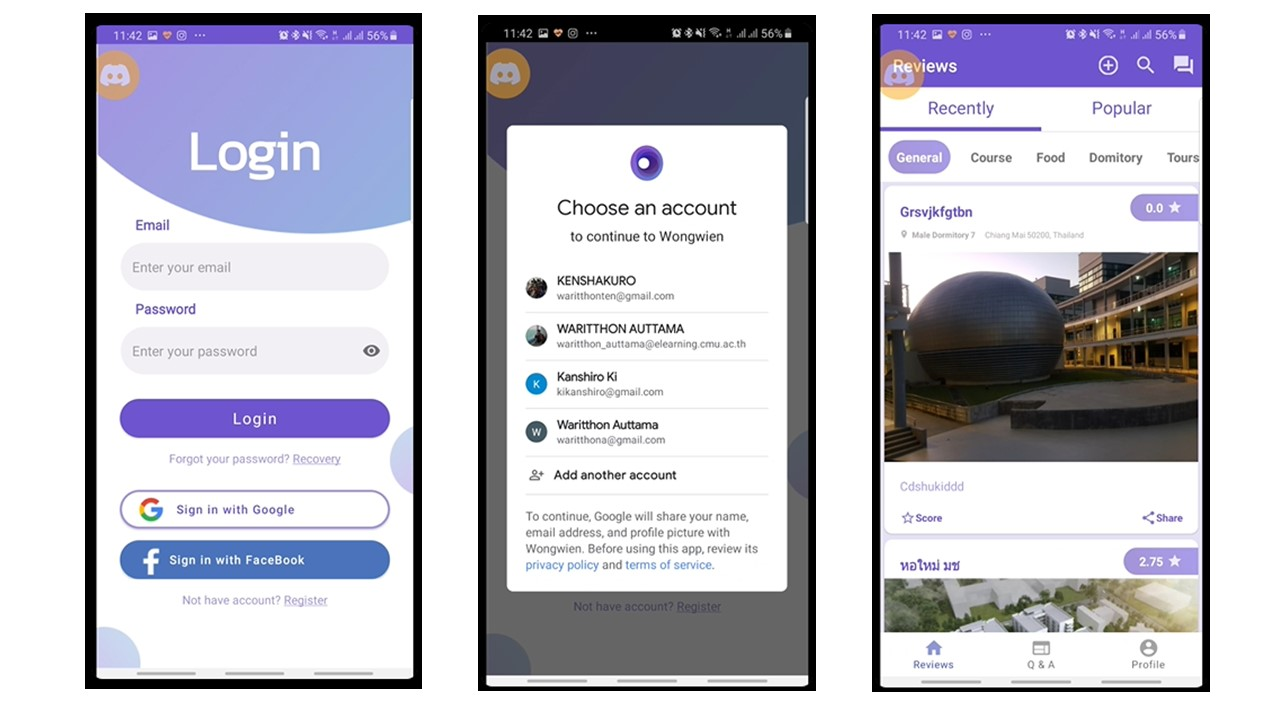
\includegraphics[width=1\textwidth]{./image/testing/Slide1.JPG}
    \end{center}
    \caption[การทดสอบโดยการการยืนยันตัวตนผ่าน google]{การทดสอบโดยการการยืนยันตัวตนผ่าน google}
    \end{figure}

\section{การทดสอบโดยการการยืนยันตัวตนผ่าน facebook}
\quad \quad  การทดสอบโดยการการยืนยันตัวตนผ่านเฟสบุ๊กโดยใช้ Facebook api เข้ามาใช้ในเขียนเชื่อมต่อ และใช้Firebase Authentication 
เข้ามาช่วยจัดการระบบหลังบ้าน (Back-end) โดยการทดลองจะยืนยันตัวตนผ่านเฟสบุ๊ก ผลลัพธ์คือสามารถเข้าสู่ระบบโดยโดยใช้บัญชีเฟสบุ๊คได้ และสามารถดึง
ข้อมูลผู้ใช้มาได้บางส่วน ดังรูป 4.2

    \begin{figure}
    \begin{center}
      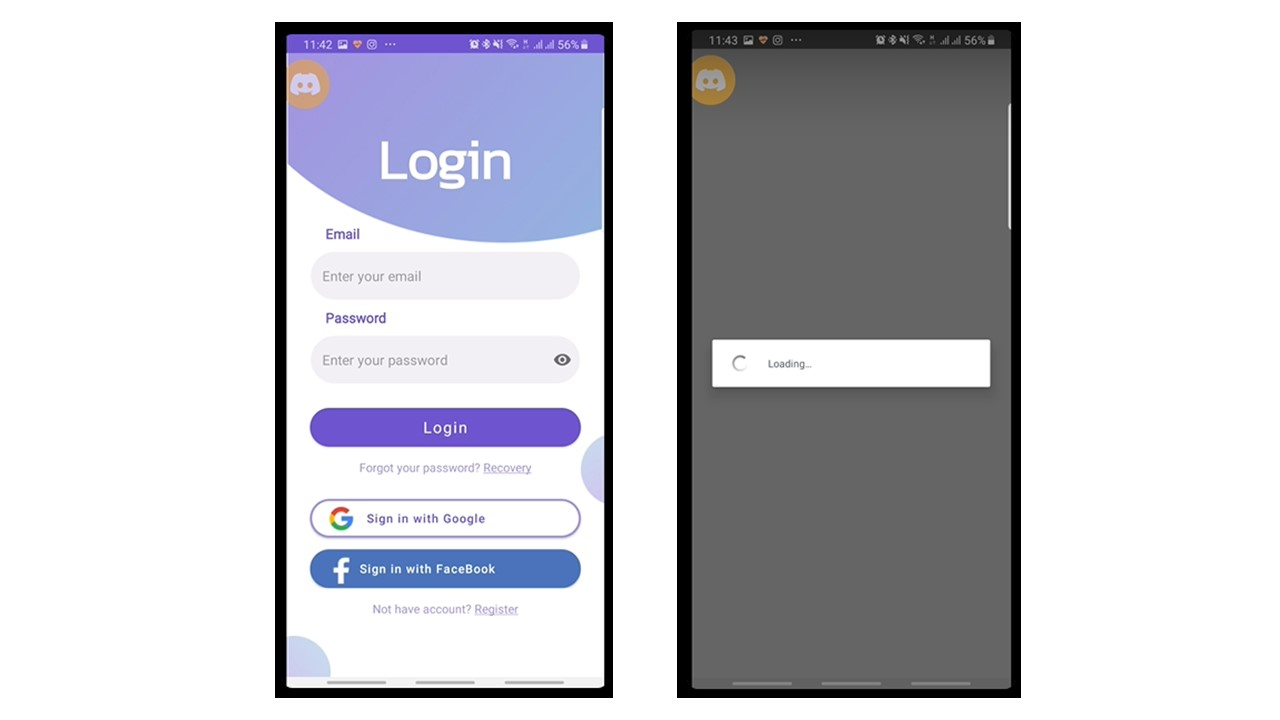
\includegraphics[width=1\textwidth]{./image/testing/Slide2.JPG}
    \end{center}
    \caption[การทดสอบโดยการการยืนยันตัวตนผ่าน facebook]{การทดสอบโดยการการยืนยันตัวตนผ่าน facebook}
    \end{figure}


\section{การทดสอบการใช้กูเกิลแผนที่ (Google map)}
\quad \quad การทดสอบเข้าใช้งาน google map โดยการจำลองการเพิ่มรีวิวได้มีการแท็กสถาที่ ซึ่งจะมาเรียกใช้งานตัว google map api เพื่อหาตำเเหน่งสถานที่ปัจจุบัน
ผลลัพธ์การทดลองคือ สามารถเข้าถึงตำแหน่งของเราปัจจุบันและสามารถดึงข้อมูลพิกัดตำแหน่งของเราได้ดังรูป 4.3
\begin{figure}
    \begin{center}
      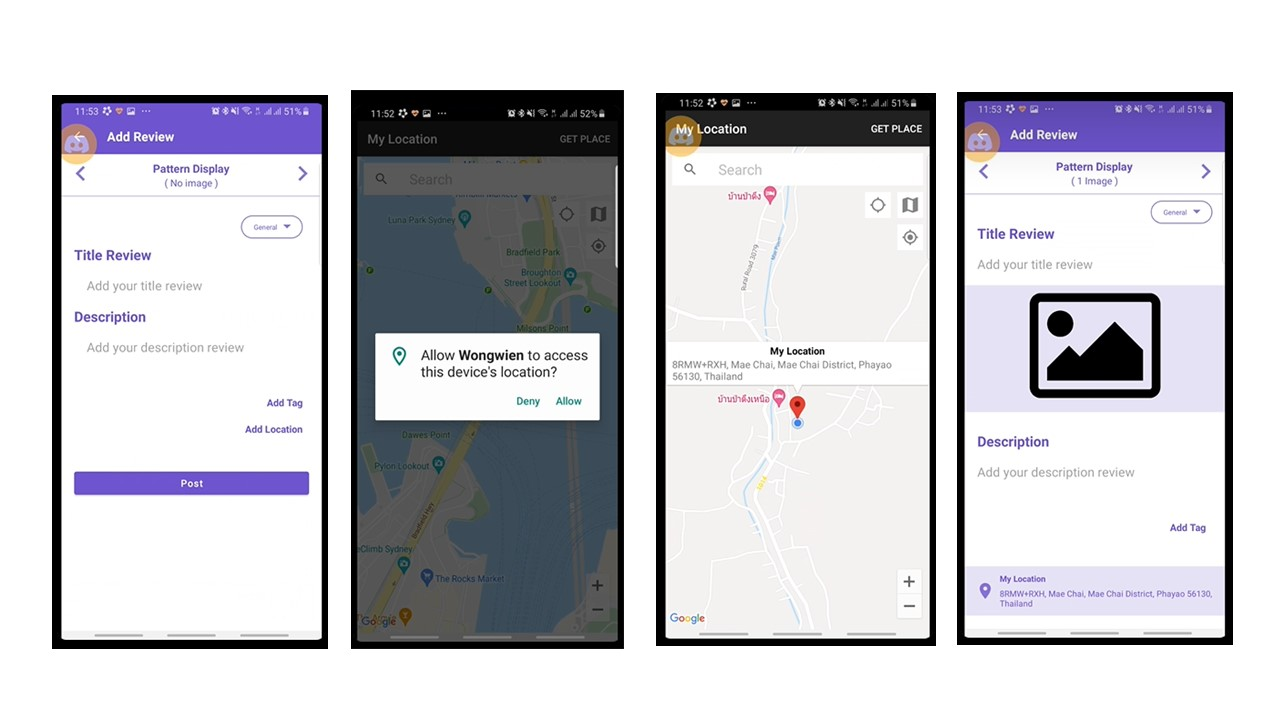
\includegraphics[width=1\textwidth]{./image/testing/Slide3.JPG}
    \end{center}
    \caption[การทดสอบการใช้กูเกิลแผนที่]{การทดสอบการใช้กูเกิลแผนที่ (Google map)}
    \end{figure}

\section{การทดสอบการเพิ่มรีวิว}
\quad \quad  การทดสอบเพิ่มการรีวิวโดยให้ทำการสร้างโฟสรีวิวขึ้นมา มีการตั้งหัวเรื่องรีวิว แนบรูป บรรยาย ติดแท็กต่างๆและมีการเเท็กสถานที่
ผลลัพธ์คือสามารถเพิ่มการรีวิวได้สำเหร็จและครบถ้วน ดังรูป 4.4
\begin{figure}
    \begin{center}
      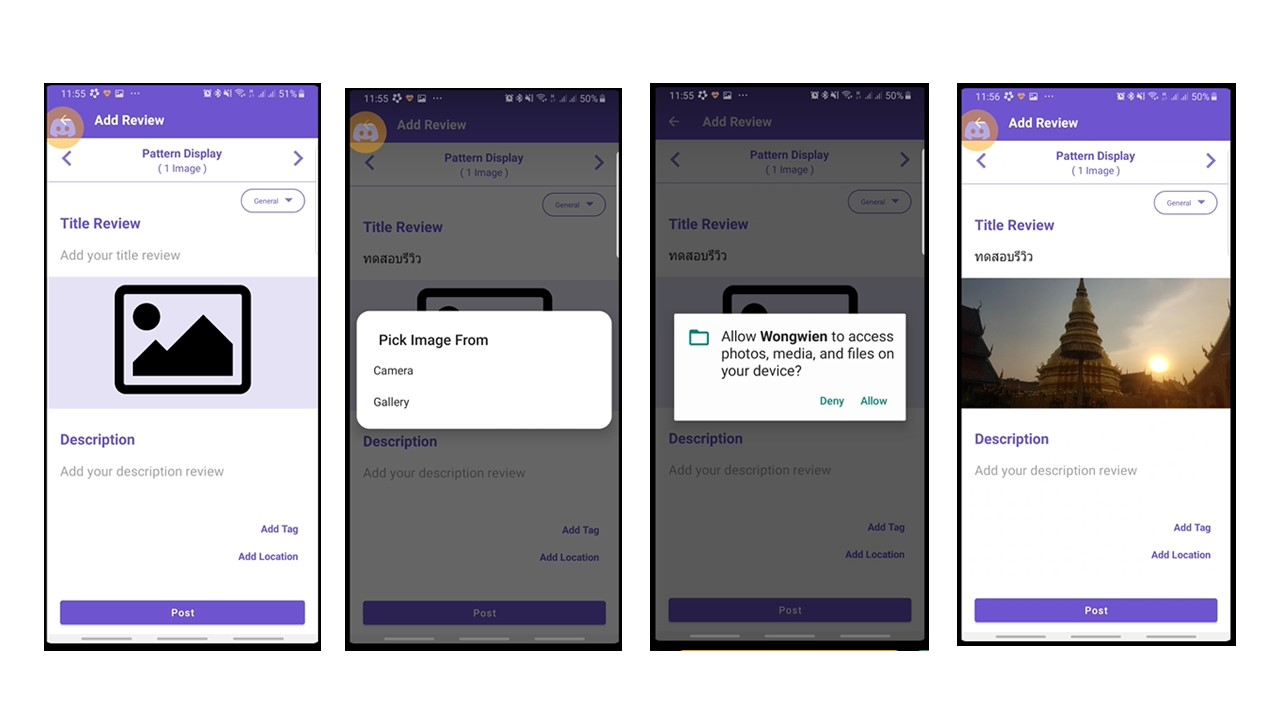
\includegraphics[width=1\textwidth]{./image/testing/Slide4.JPG}
    \end{center}
    \end{figure}

    \begin{figure}
        \begin{center}
          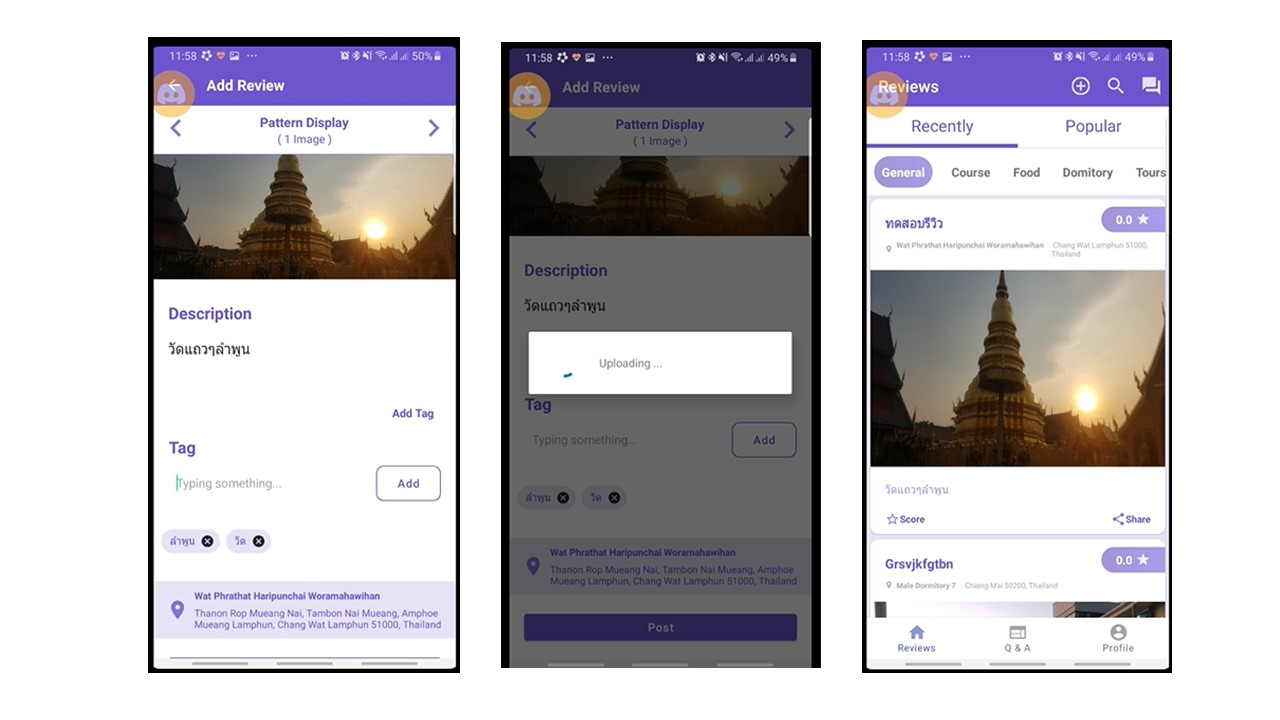
\includegraphics[width=1\textwidth]{./image/testing/Slide5.JPG}
        \end{center}
        \caption[การทดสอบการเพิ่มรีวิว]{การทดสอบการเพิ่มรีวิว}
        \end{figure}

\section{การทดสอบการให้คะแนนรีวิว}
\quad \quad การทดสอบการให้คะแนนรีวิว โดยให้ทำการให้คะแนนดาวรีวิว การคำนวนคะแนนรีวิวมาจากการเฉลี่ยของคนที่ให้ตะแนนรีวิว
ผลการทดสอบคือสามารถให้คะแนนดาวรีวิวได้สำเหร็จและคำนวนได้ถูกต้องดังรูป 4.5
\begin{figure}
    \begin{center}
      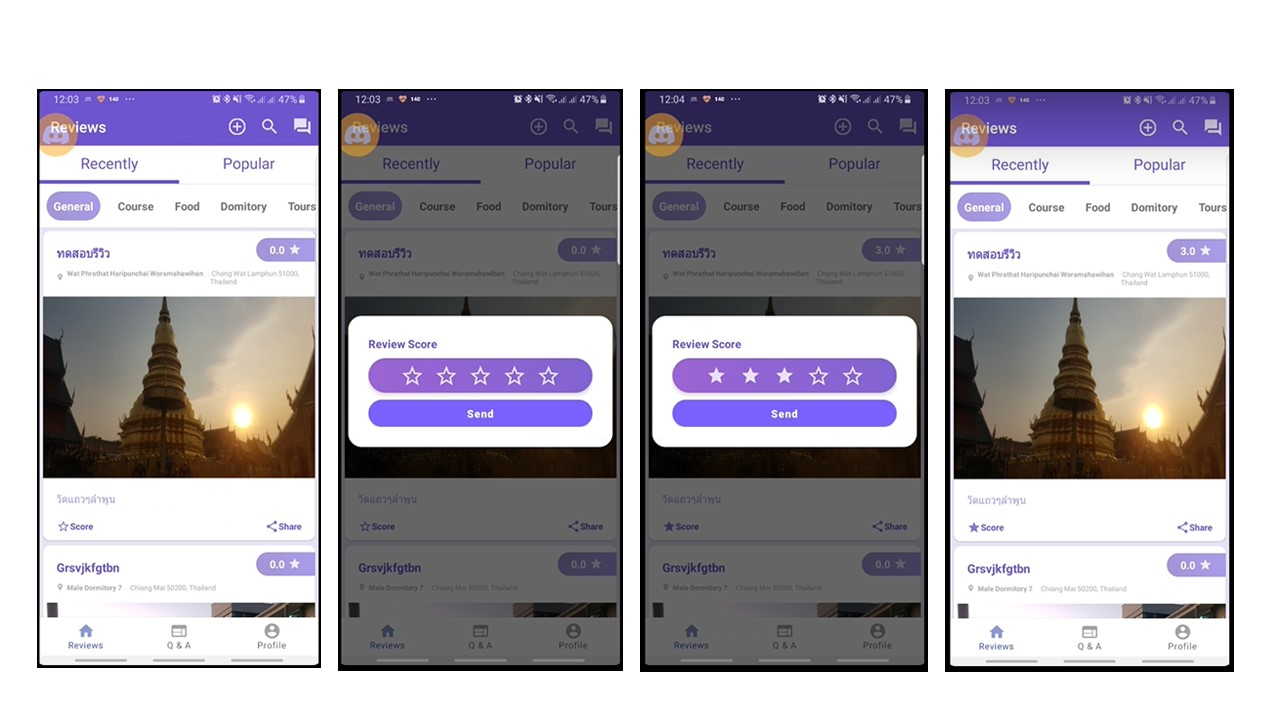
\includegraphics[width=1\textwidth]{./image/testing/Slide6.JPG}
    \end{center}
    \caption[การทดสอบการให้คะแนนรีวิว]{การทดสอบการให้คะแนนรีวิว}
    \end{figure}

\section{การทดสอบการให้คอมเม้น}
\quad \quad การทดสอบการให้คอมเม้น คือจะให้เข้าไปคอมเม้นในส่วนของรีวิวโดยเลือกรีวิวมาแล้วกดเข้าไปดุรายละเอียดของรีวิวจากนั้นก็
สามารถคอมเม้นรีวิวนั้นๆ ผลลัพธ์คือสามารถคอมเม้นได้สำเหร็จระบบก็จะแสดงคอมเม้นล่าสุดที่เราพึ่งคอมเม้นไป ดังรูป 4.6 

\begin{figure}
    \begin{center}
      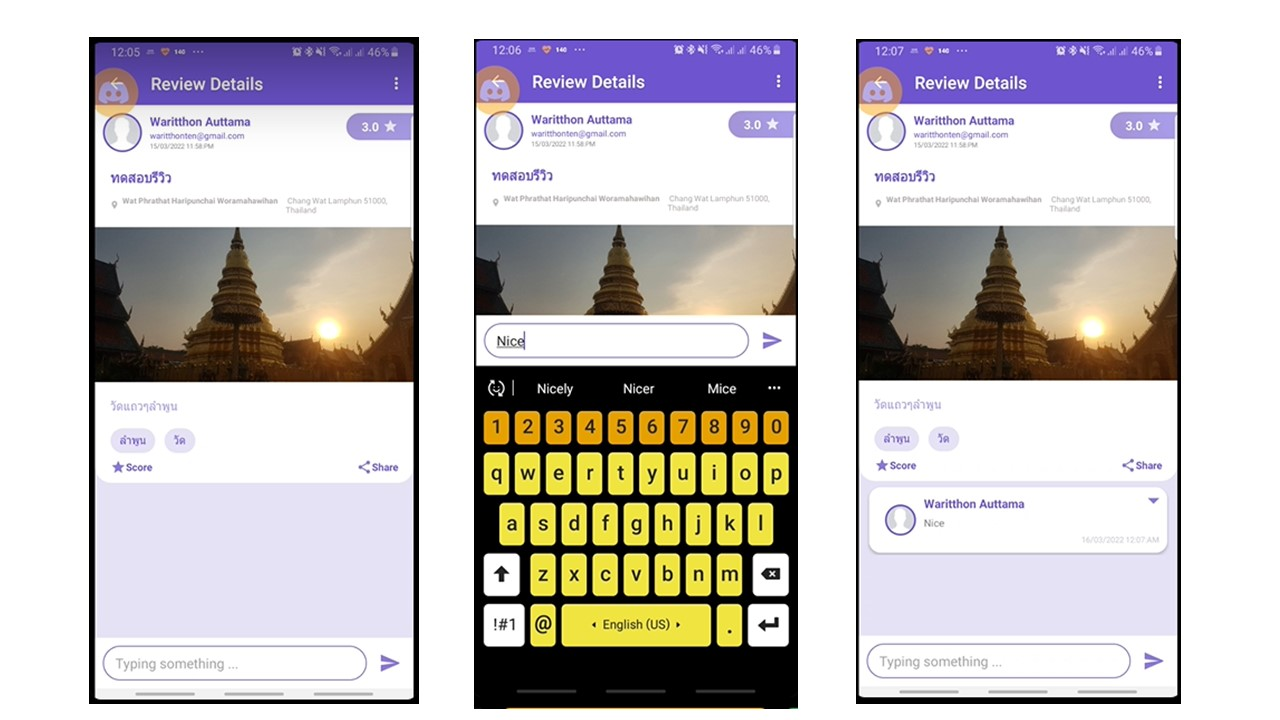
\includegraphics[width=1\textwidth]{./image/testing/Slide7.JPG}
    \end{center}
    \caption[การทดสอบการให้คอมเม้น]{การทดสอบการให้คอมเม้น}
    \end{figure}

\section{การทดสอบการแก้ไขคอมเม้น}
\quad \quad การทดสอบการแก้ไขคอมเม้น คือจะให้เข้าไปแก้ไขคอมเม้นที่เราได้คอมเม้นไปจากการทดลองก่อนหน้านี้ โดยการแก้ไขคือให้กดคอมเม้นที่เราคอมเม้นไปค้างไว้สักพักจะปรากฎเมนูแก้ไขขึ้นมา
ให้เราทำการพิมแก้ไขคอมเม้นรีวิว จกานั้นกดปุ่ม update ผลลัพธ์คือสามารถแก้ไขคอมเม้นได้สำเหร็จ ระบบก็จะแสดงคอมเม้นล่าสุดที่เราพึ่งแก้ไขคอมเม้นไป ดังรูป 4.7 

\begin{figure}
    \begin{center}
      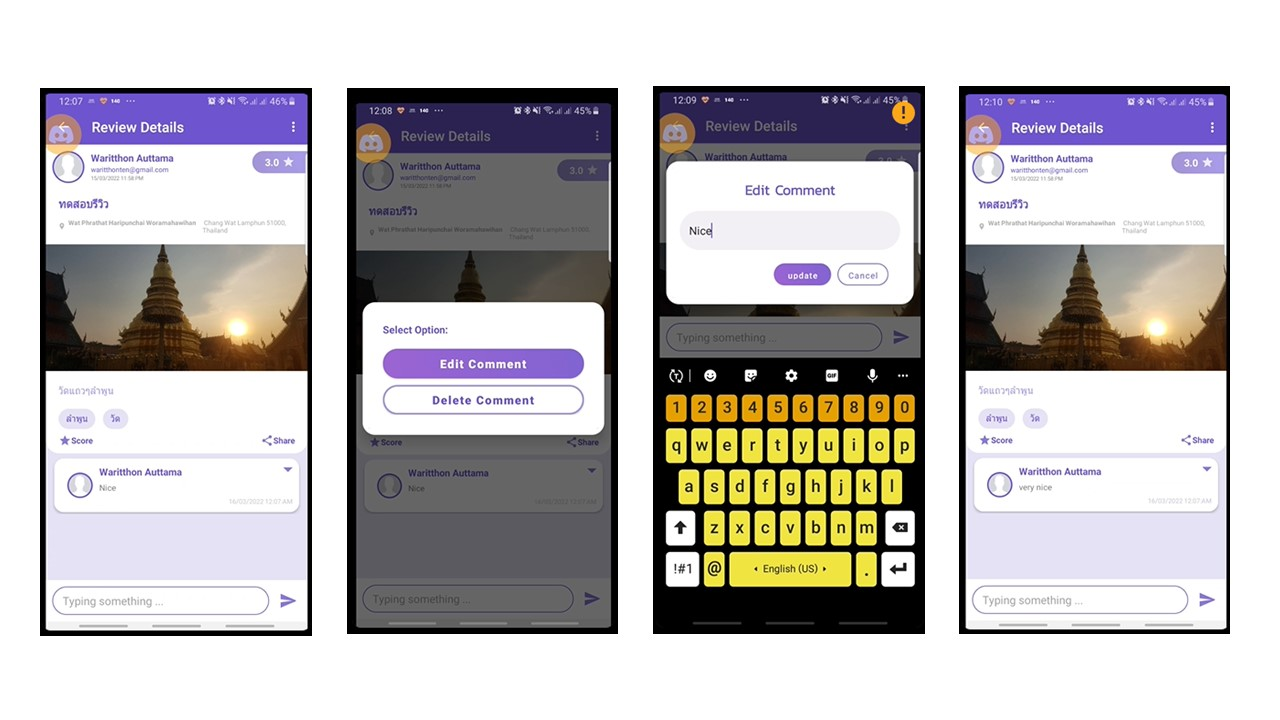
\includegraphics[width=1\textwidth]{./image/testing/Slide8.JPG}
    \end{center}
    \caption[การทดสอบการแก้ไขคอมเม้น]{การทดสอบการแก้ไขคอมเม้น}
    \end{figure}
    
\section{การทดสอบการเพิ่มกระทู้}
\quad \quad การทดสอบการเพิ่มกระทู้ คือจะให้เปิดหน้ากระทู้จากนั้นกดปุ่ม + เพื่อเพิ่มการตั้งกระทู้ เมื่อตั้งกระทู้แล้วกดปุ่มโฟส 
ผลลัพธ์คือสามารถเพิ่มกระทู้ได้สำเหร็จ ระบบจะแสดงกระทู้ล่าสุดที่เราพึ่งโฟสไป  ดังรูป 4.8

\begin{figure}
    \begin{center}
      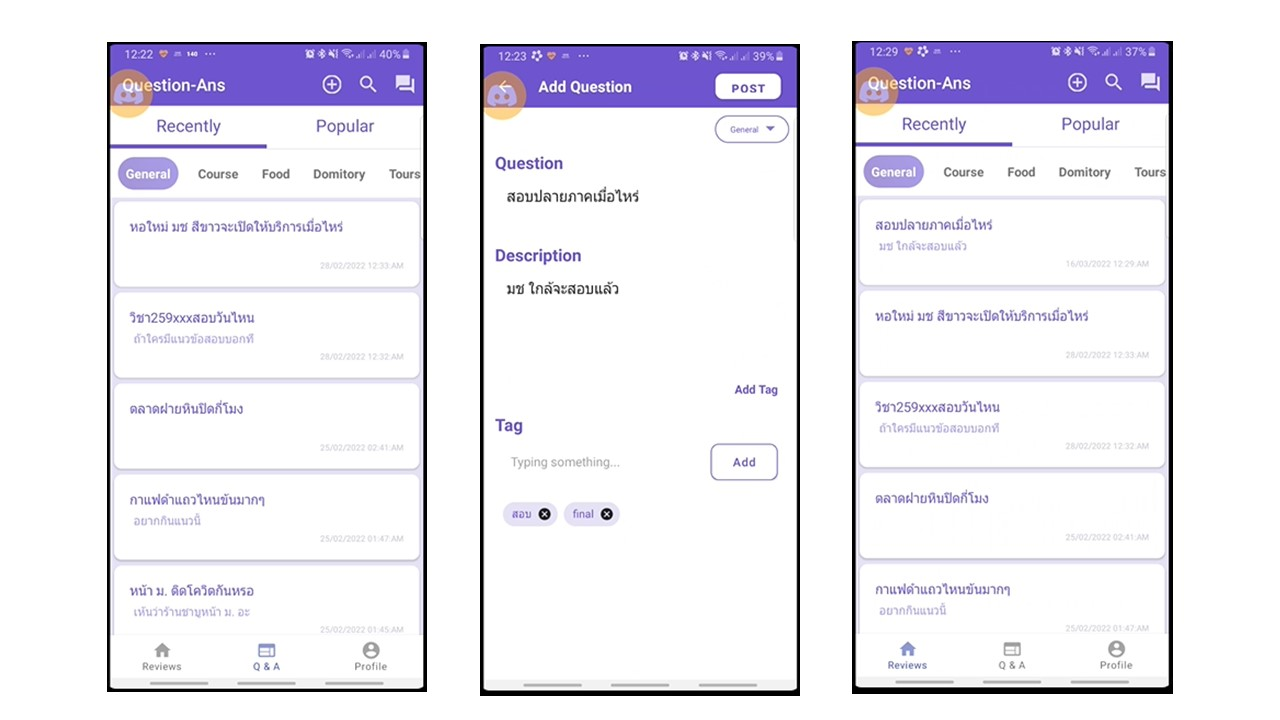
\includegraphics[width=1\textwidth]{./image/testing/Slide9.JPG}
    \end{center}
    \caption[การทดสอบการเพิ่มกระทู้]{การทดสอบการเพิ่มกระทู้}
    \end{figure}

\section{การทดสอบการเพิ่ม usefull comment}
\quad \quad การทดสอบการเพิ่ม usefull comment คือจะเป็นฟังชั่นที่ช่วยแนะนำผู้ที่เข้ามาอ่านกระทู้ได้เข้าใจง่ายๆว่ากระทู้นี้ มีคอมเม้นนี้ที่สามารถช่วยในการแก้ไขปัญหาหรือ
ช่วยแนะนำได้ดี โดยสามารถเพิ่ม usefull comment ได้ก็ต่อเมื่อเป็นเจ้าของกระทู้ เจ้าของกระทู้จะมีเมนูของคอมเม้นปรากฎอยู่เมื่อกดเข้าไปจะแสดงเมนู add usefull comment 
ผลลัพธ์คือสามารถเพิ่ม usefull comment ได้สำเหร็จ ระบบจะมีการแสดงสีของ usefull commentที่ต่างออกไปเพื่อให้มองเห็นได้ง่าย  ดังรูป 4.9

\begin{figure}
    \begin{center}
      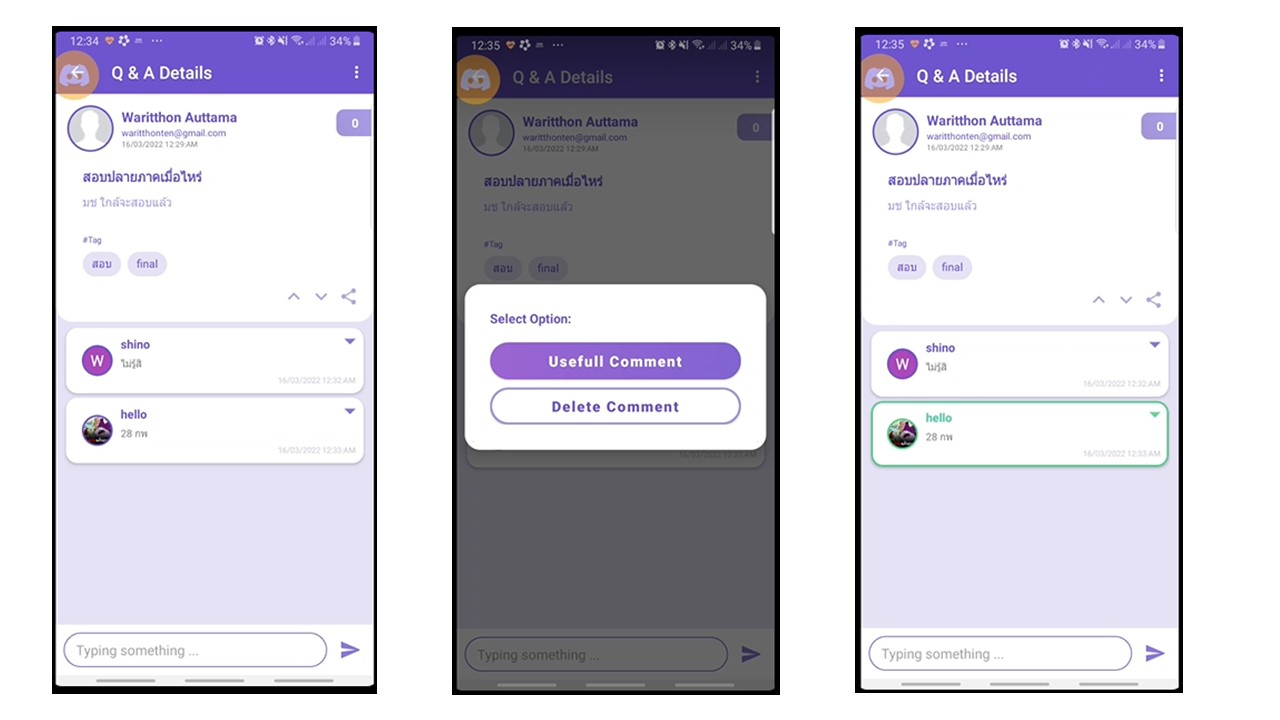
\includegraphics[width=1\textwidth]{./image/testing/Slide10.JPG}
    \end{center}
    \caption[การทดสอบการเพิ่ม usefull comment]{การทดสอบการเพิ่ม usefull comment}
    \end{figure}

\section{การทดสอบการค้นหารีวิว}
\quad \quad การทดสอบการค้นหารีวิว คือฟังชั่นที่สามารถพิมค้นรีวิวหรือกระทู้ก็ได้ โดยการทดลองจะให้พิมค้นหารีวิว hello  
ผลลัพธ์คือระบบจะแสดงรายการที่มีชื่อหรือมีส่วนเกี่ยวข้องกับ hello คำค้นของเรา  ดังรูป 4.10

\begin{figure}
    \begin{center}
      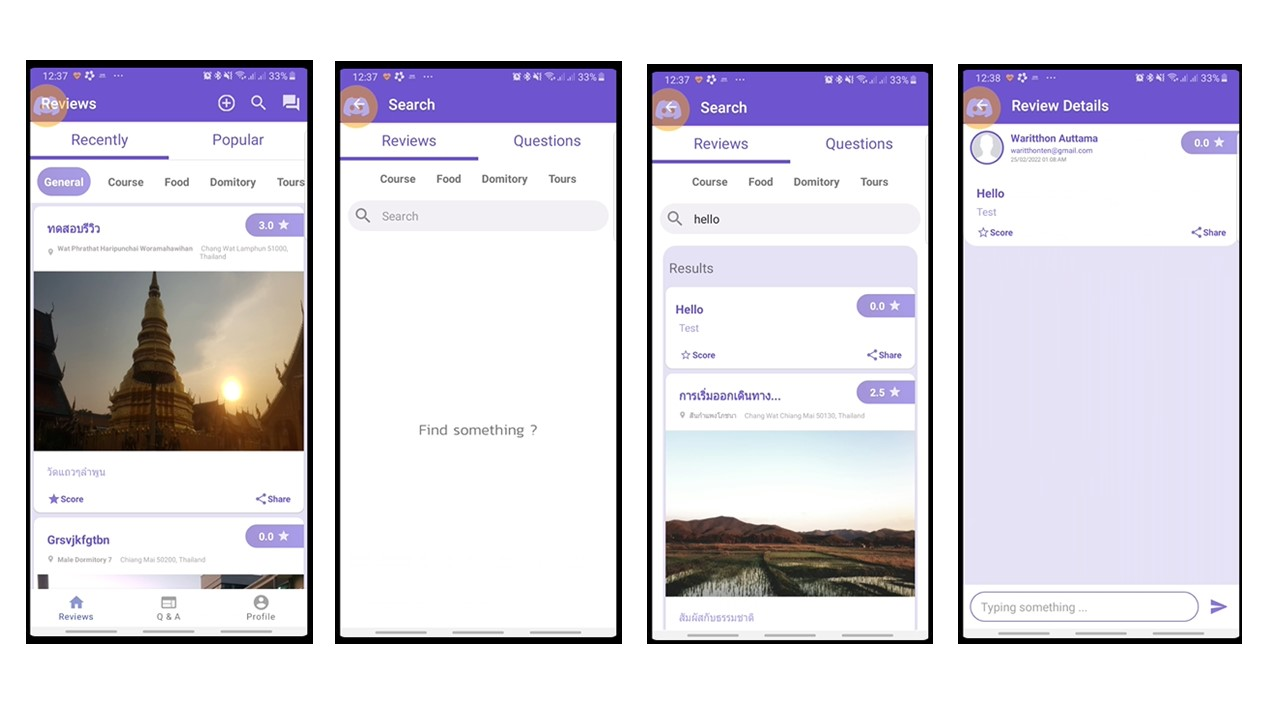
\includegraphics[width=1\textwidth]{./image/testing/Slide11.JPG}
    \end{center}
    \caption[การทดสอบการค้นหารีวิว]{การทดสอบการค้นหารีวิว}
    \end{figure}

\section{การทดสอบการหาเพื่อนและเริ่มการสนทนา}
\quad \quad การทดสอบการหาเพื่อนและเริ่มการสนทนา คือเราสามารถค้นหาเพื่อนที่เราจะเริ่มคุยด้วยได้จากชื่อหรืออีเมล
ผลลัพธ์คือระบบสามารถทำงานค้นหาได้อย่างถูกต้องและสามารถส่งข้อความหาคู่สนทนาได้  ดังรูป 4.11

\begin{figure}
    \begin{center}
      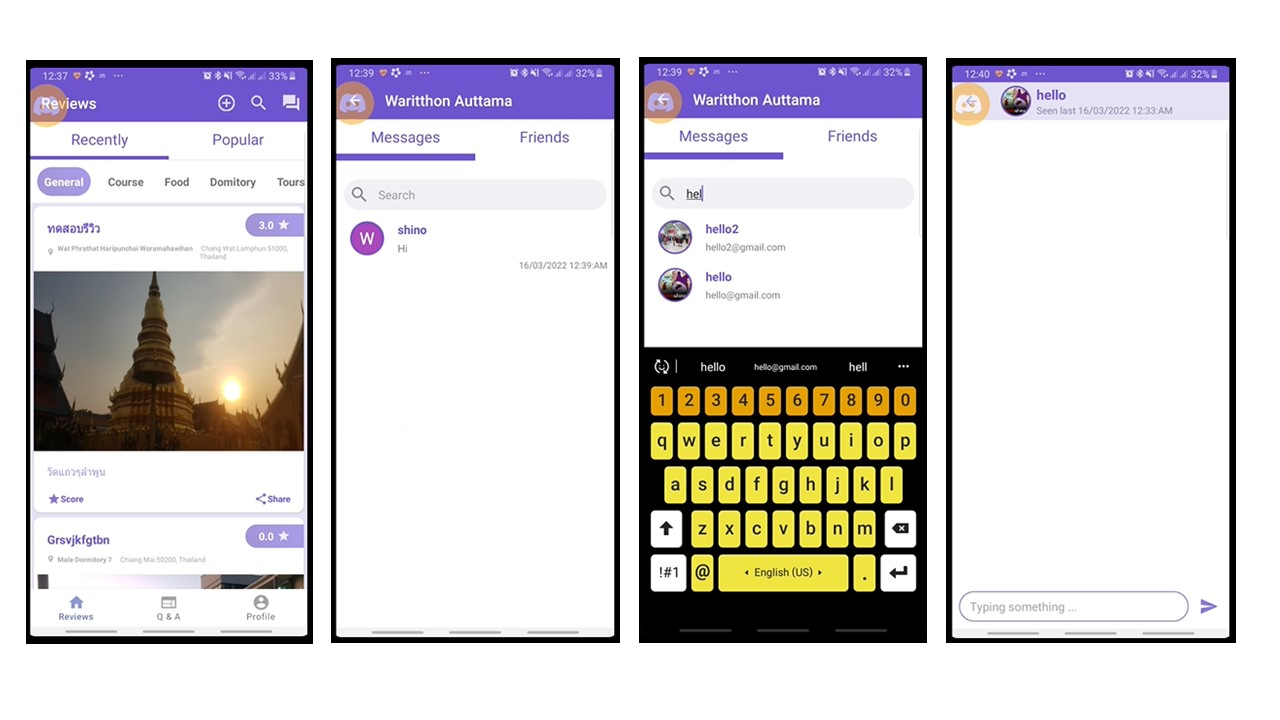
\includegraphics[width=1\textwidth]{./image/testing/Slide12.JPG}
    \end{center}
    \end{figure}

\begin{figure}
    \begin{center}
      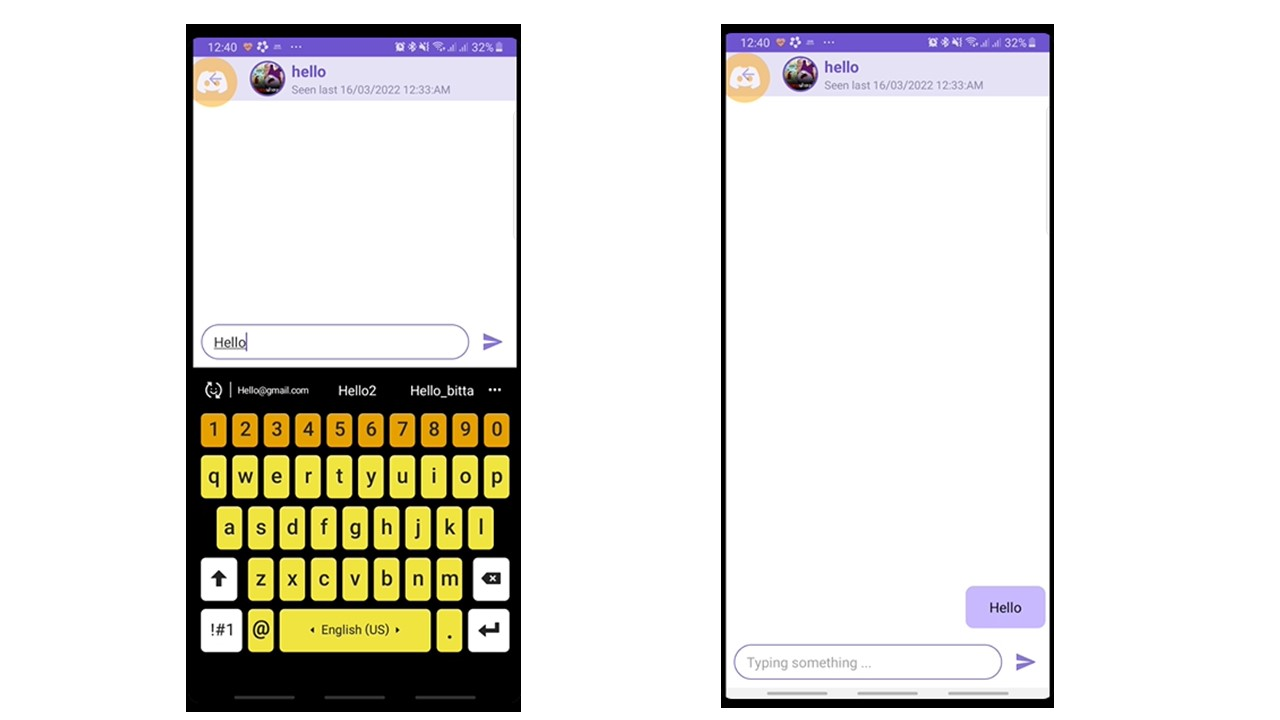
\includegraphics[width=1\textwidth]{./image/testing/Slide13.JPG}
    \end{center}
    \caption[การทดสอบการหาเพื่อนและเริ่มการสนทนา]{การทดสอบการหาเพื่อนและเริ่มการสนทนา}
    \end{figure}
\ifproject
\chapter{\ifenglish Conclusions and Discussions\else บทสรุปและข้อเสนอแนะ\fi}

\section{\ifenglish Conclusions\else สรุปผล\fi}

จากการพัฒนาโครงงาน Wongwien ระบบที่ได้สามารถทำงานตามวัตถุประสงค์ของโครงงานได้นั่นคือได้แพลตฟอร์มที่สามารถใช้ใน
การรีวิวเรื่องต่างๆต่างหมวดหมู่ สามารถตั้งกระทู้เพื่อไขข้อสงสัยต่างๆ สามารถค้นหารีวิวได้อย่างรวดเร็ว สามารถสนทนาขอรับคำปรึกษาและ
สามารถเพิ่มวิธีการเข้าใช้งานระบบผ่านแฟตฟอร์มอื่นเพื่อความสะดวกสบาย

จากผลการทดสอบกับผู้ใช้งานสรุปได้ดังนี้
ระบบสามารถทำงานต่างๆได้ดีโดยรวม ปัญหาที่พบระหว่างการทดสอบความหน่วงที่เกิดจาการดึงข้อมูลมาแสดงผล ผู้ใช้งานสามารถใช้
งานแอพพลิเคชันโดยไม่เกิดความสับสน


\section{\ifenglish Challenges\else ปัญหาที่พบและแนวทางการแก้ไข\fi}

ในการทำโครงงานนี้ พบว่าเกิดปัญหาหลักๆ ดังนี้
\begin{enumerate}
    \item ปัญหาด้านการทดสอบระบบ อันเนื่องมาจากสถานการณ์โรคระบาดโควิด-19ทำให้การทดสอบระบบต้องทดสอบด้วยความล่าช้า
    เนื่องจากไม่ได้ทำเรื่องเบิกเงินเพื่อสมัครสมาชิกนำแอพขึ้น play store ทำให้ต้องใช้การติดตั้งแบบ apk ไฟล์ผ่าน android studio
    โดยต้องนัดเจอกันเพื่อติดตั้งแอพทดสอบ สถานการณ์โรคระบาดโควิด-19ทำให้การนัดเจอกันค่อนข้างยากขึ้น
    \item การทำงานของแอพพลิเคชันเมื่อมีอินเตอร์เน็ตที่ช้าทำให้การดึงข้อมูลช้าตามอาจสร้างความลำคาญกับผู้ใช้ได้
    \item ในการทำโปรเจคในครั้งนี้เรื่องของการแชร์ไปยังแอปพลิเคชันอื่นรอรับการแชร์ที่สมบูรณ์เมื่อเเชร์ผ่านอีเมล
    \item ระบบสามารถทำงานแบบออฟไลน์ได้ถ้าหากเคยมีการใช้งานมาก่อนจะเก็บเนื้อหาล่าสุดไว้
\end{enumerate}
\section{\ifenglish%
Suggestions and further improvements
\else%
ข้อเสนอแนะและแนวทางการพัฒนาต่อ
\fi
}

ข้อเสนอแนะเพื่อพัฒนาโครงงานนี้ต่อไป มีดังนี้
\begin{enumerate}
    \item ควรทำการพัฒนา UI ให้สวยงามน่าใช้งานมากกว่านี้และควรมีฟังชันอื่นๆที่น่าสนใจเพื่อดึงดูดผู้ใช้งาน
    \item ควรเพิ่มความสามารถในการปรับแต่งการรีวิวให้มันมีมากกว่านี้
\end{enumerate}

\fi

\bibliography{sampleReport}

\ifproject
\appendix
\chapter{แบบฟอร์มสอบถามความพึงพอใจในการใช้งานแอปพลิเคชัน}

% Text for the first appendix goes here.

% \section{Appendix section}

แบบสอบถามความพึงพอใจหลังทดลองใช้งานแอปพลิเคชัน

\begin{figure}
  \begin{center}
    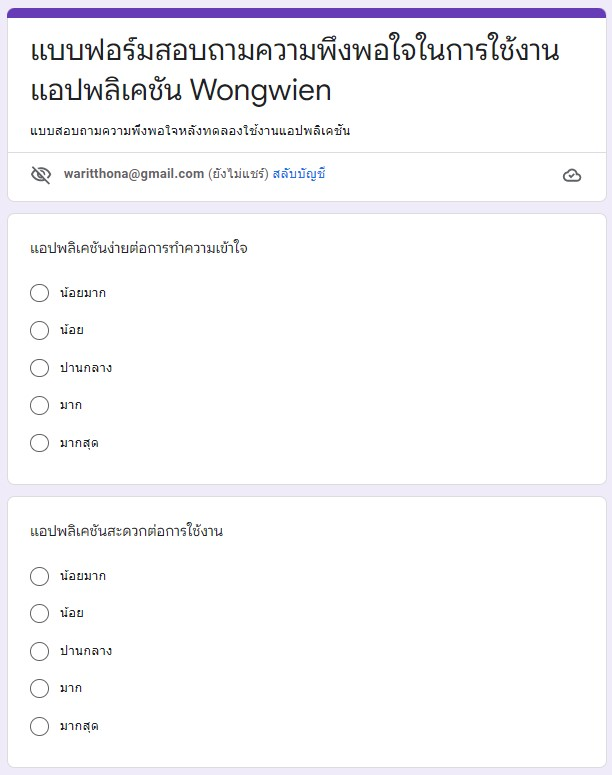
\includegraphics[width=1\textwidth]{./image/form/form1.jpg}
  \end{center}
  \end{figure}

\begin{figure}
  \begin{center}
    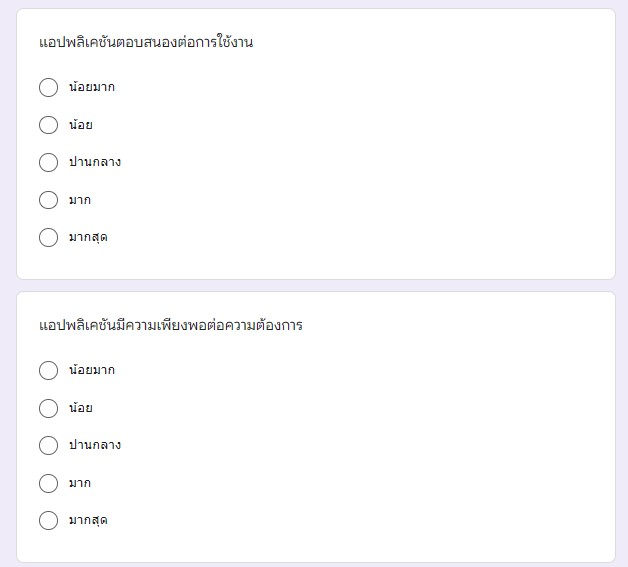
\includegraphics[width=1\textwidth]{./image/form/form2.jpg}
  \end{center}
  \end{figure}

\begin{figure}
  \begin{center}
    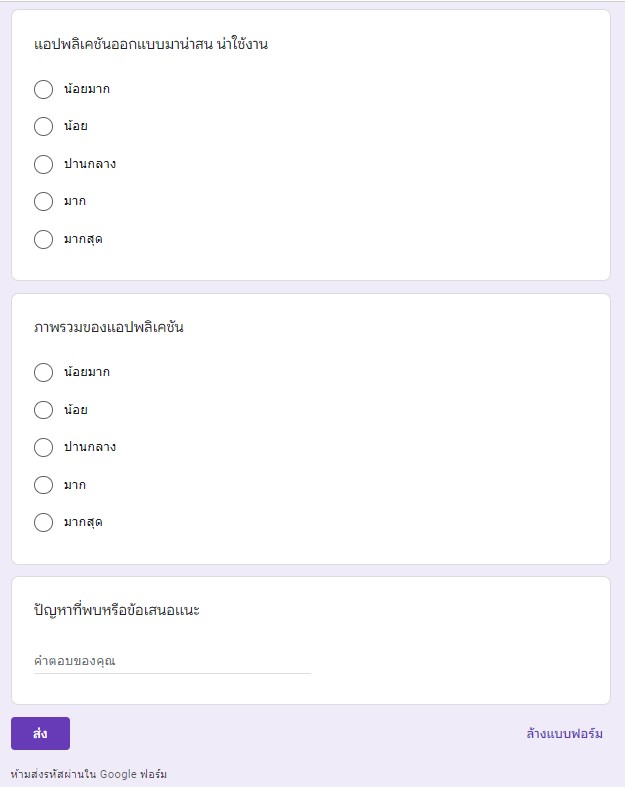
\includegraphics[width=1\textwidth]{./image/form/form3.jpg}
  \end{center}
  \caption[แบบสอบถามความพึงพอใจหลังทดลองใช้งานแอปพลิเคชัน]{แบบสอบถามความพึงพอใจหลังทดลองใช้งานแอปพลิเคชัน}
  \end{figure}
% test ทดสอบฟอนต์ serif

% \textsf{test ทดสอบฟอนต์ sans serif}

\ifenglish\else
% TODO: Thai teletype font still doesn't work with english option
% \verb+test ทดสอบฟอนต์ teletype ภาษาไทย+

% \texttt{test ทดสอบฟอนต์ teletype ภาษาไทย}
\fi

\chapter{\ifenglish Manual\else คู่มือการใช้งานระบบ\fi}

\subsection{คู่มือการติดตั้ง }

สามารถศึกษาวิธีการติดตั้งได้จากลิงค์ต่อไปนี้

github: \href{https://github.com/tenshiro007/wongwien_project}{https://github.com/tenshiro007/wongwien\_project}

\subsection{ขั้นตอนการเข้าใช้งาน }

เมื่อทำการเข้าสู่ระบบเราแอพจะนำเราไปสู่หน้า dashboard โดยสามารถเลือกไปยัง dashboardต่างๆได้ เช่น Q-A dashboard, Review
dashboard ,Profile dashboard นอกจากนี้เมนูบาร์ข้างบนจะมีไอคอนที่จะนำพาเราไปยังหน้าของการค้นหาและระบบแชท โดยในส่วนของ
หน้าค้นหาเราสามารถเลือกค้นหารีวิวหรือกระดานตั้งกระทู้ก็ได้ และในส่วนของระบบแชทจะนำเราไปสู่หน้าข้อมูลการสนทนาล่าสุด สามารถ
ค้นหาเพื่อน และเริ่มการสนทนาได้
 \begin{figure}[h]
\begin{center}
  \includegraphics[width=1\textwidth]{./image/reviews/howtouse.JPG}
\end{center}  
\end{figure}

สามารถดูคู่มือการใช้งานระบบได้จากลิงค์ต่อไปนี้

เอกสารนำเสนอ:\href{www.canva.com/design/DAEschMH9Gk/tpbr2nRzCNLEltHK_8zbpA/view/}{www.canva.com/design/DAEschMH9Gk/tpbr2nRzCNLEltHK\_8zbpA/view/}

youtube : \href{https://www.youtube.com/watch?v=Zabpci5Do2c}{https://www.youtube.com/watch?v=Zabpci5Do2c}

%% Display glossary (optional) -- need glossary option.
\ifglossary\glossarypage\fi

%% Display index (optional) -- need idx option.
\ifindex\indexpage\fi

\begin{biosketch}
\begin{center}
  % 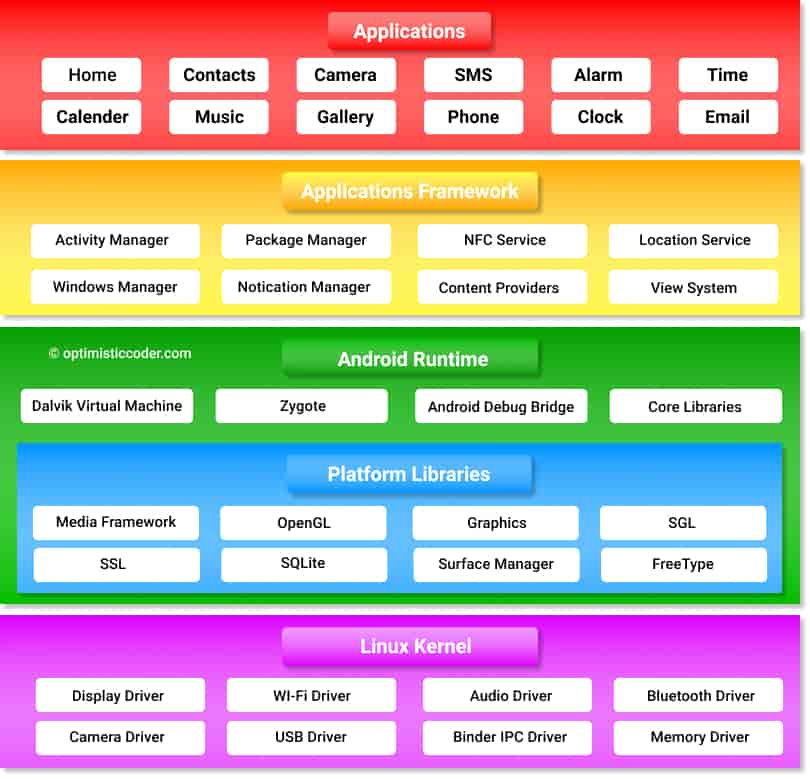
\includegraphics[width=0.8\textwidth]{./image/architecture.jpg}
  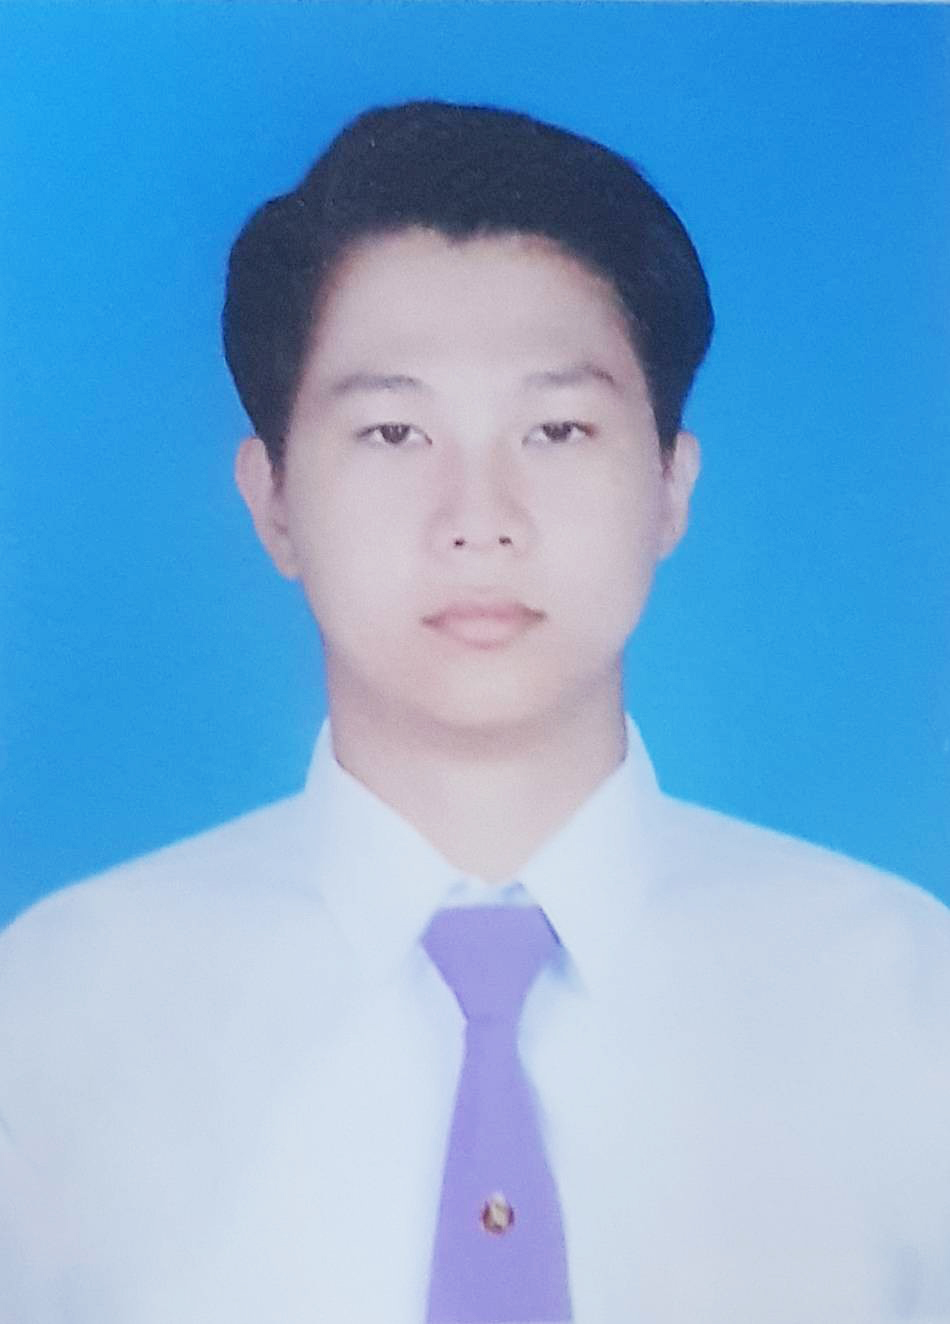
\includegraphics[width=1.5in]{./image/profile.jpg}
\end{center}
นาย วริทธิ์ธร อุตตะมา เกิดวันที่ 17 พฤศจิกายน 2542 ณ จังหวัด พะเยา สำเร็จการศึกษา
ระดับมัธยมจากโรงเรียนพะเยาพิทยาคม เข้าศึกษาที่ภาควิชาวิศวกรรมศาสตร์ สาขาคอมพิวเตอร์
มหาวิทยาลัยเชียงใหม่ เมื่อ พฤษภาคม 2561 โดยมีความสนใจเป็นพิเศษในด้านการพัฒนาแอปพลิเคชัน
มือถือและเว็บไซต์

% the \texttt{biosketch} environment.
\end{biosketch}
\fi % \ifproject
\end{document}
